% \documentclass[pageno,hyperref]{jpaper}
\documentclass{article}

\usepackage[disable]{todonotes}
\usepackage[binary-units,per-mode=symbol]{siunitx}
% \usepackage[binary-units,per-mode=symbol]{SIunits}
\usepackage{tikz}
\usetikzlibrary{positioning, fit, calc, shapes, arrows}
\usepackage{pgfplots}
\usepackage[section]{placeins}
\usepackage{outlines}
\usepackage{bytefield}
\usepackage[underline=false]{pgf-umlsd} 
\usepackage[toc, acronym, nopostdot]{glossaries}
\usepackage{xparse}
\usepackage[normalem]{ulem}
\usepackage{listings}

\usetikzlibrary{patterns}
\graphicspath{ {./figs/} }
\pgfplotsset{compat=1.13}
\makeglossaries


% For stuff that's both an acryonym and a glossary entry
\newcommand*{\newdualentry}[5][]{%  
  \newglossaryentry{main-#2}{name={#4},%  
  text={#3\glsadd{#2}},%  
  description={#5},%  
  #1  
  }%  
  \newacronym{#2}{#3\glsadd{main-#2}}{#4}%  
}

% \glsdisablehyper
\renewcommand*{\glstextformat}[1]{\textcolor{black}{#1}}

\newdualentry{wsc}
  {WSC}
  {warehouse-scale computer}
  {Generic term referring to tightly-integrated clusters of
    machines deployed in the data center.}

\newdualentry{sip}
  {SiP}
  {system in package}
  {A system where all the necessary components (NIC, cpu, memory)
   are grouped into the same physical package (but not necessarily on the same
   chip)}

\newglossaryentry{paging}
{
  name={paging},
  description={The process of storing logical pages on an external storage
device in order to free physical memory. Also called "swapping".}
}

\newdualentry{pfa}
  {PFA}
  {page fault accelerator}
  {The proposed hardware-accelerator that handles page-faults for
  remote pages automatically.}

\newglossaryentry{disag}
{
  name={dissaggregation},
  description={The WSC design that moves compute resources (such as memory,
disk, and CPUs) into dedicated resource-blades that are connected through a
high-performance network.}
}

\newdualentry{numa}
  {NUMA}
  {non-uniform memory access}
  {A system where memory is cache-coherently available to multiple CPUS, but
   with varying access latencies and bandwidths (a type of multi-socket
   machine).}

\newdualentry{rdma}
  {RDMA}
  {remote direct memory access}
  {A system where memory is directly addressable between multiple
   nodes through a network interface. RDMA systems are not typically
   cache-coherent.}

\newglossaryentry{page}
{
  name={page},
  description={A fixed-size logical group of data (typically
\SI{4}{\kibi\byte}). Sometimes called ``virtual page''.}
}

\newglossaryentry{page frame}
{
  name={page frame},
  description={A fixed-size region of physical memory used to store pages.}
}

\newglossaryentry{frame}
{
  name={frame},
  description={Synonym for page frame},
  see=[Glossary:]{page frame}
}

\newglossaryentry{pgtbl}
{
  name={page table},
  description={A hardware-visible tree in main memory that contains
translations from virtual to physical addresses.}
}

\newdualentry{pte}
  {PTE}
  {page table entry}
  {A single entry of the page-table. Each PTE refers to a single
  virtual page.}

\newdualentry{tlb}
  {TLB}
  {translation look-aside buffer}
  {A cache of virtual to physical address translations.}

\newdualentry{ptw}
  {PTW}
  {page table walker}
  {A hardware device to automatically walk the page-table and
  locate PTEs for a particular virtual address.}

\newglossaryentry{bookkeeping}
{
  name={bookkeeping},
  description={The internal OS-specific tasks related to bringing in a new
page. This typically includes updating meta-data and other page-tracking
activities.}
}

\newglossaryentry{freeq}
{
  name={FreeQ},
  description={Queue of free frames to be used by the PFA to service
page-faults.}
}

\newglossaryentry{newq}
{
  name={NewQ},
  description={Queue of new-page descriptors populated by the PFA on every page
fault and drained by the OS for bookkeeping.}
}

\newglossaryentry{evictq}
{
  name={EvictQ},
  description={Queue of pages to be evicted by the PFA. Populated by the OS
when it needs to free local physical memory.}
}

\newglossaryentry{pgid}
{
  name={pageID},
  description={A unique identifier for a page in remote memory. Acts as a
remote-memory address.}
}

\newglossaryentry{memory blade}
{
  name={memory blade},
  description={A dedicated memory node in a disaggregated system. The memory blade
exists solely to server memory requests. A memory blade may be custom-designed
for this purpose, or may simply expose an RDMA interface.}
}

\newdualentry{mtu}
  {MTU}
  {maximum transfer unit}
  {The largest contiguous packet that a network is capable of
  transmitting.}

\newdualentry{tmem}
  {TMem}
  {transcendent memory}
  {A layer in the Linux paging subsystem that stores pages in
  specialized memory that may not be disk-backed.}

\newglossaryentry{cgroup}
{
  name={cgroup},
  first={control group (cgroup)},
  description={The per-task (or group of tasks) resource management system in
the Linux kernel.}
}

\newglossaryentry{swap}
{
  name={swap},
  description={Historically used to refer to the process of moving an entire
process's memory image to disk, Linux uses ``swapping'' to refer to all
paging.}
  see=[Glossary:]{paging}
}

\newglossaryentry{anonpg}
{
  name={anonymous page},
  description={A page that does not contain disk-backed information. This is
primarily ``heap'' memory (e.g. memory allocated through malloc())}
}

\newdualentry{vma}
  {VMA}
  {virtual memory area}
  {Contiguous region of virtual memory used by Linux to simplify memory
   management.}

\newglossaryentry{swpent}
{
  name={swap\_entry\_t},
  description={A Linux-specific value stored in evicted PTEs that contains
information on where to locate an evicted page.}
}

\newglossaryentry{kpfad}
{
  name={kpfad},
  description={A background daemon that opportunistically performs bookkeeping
  and maintenance for the PFA.}
}

\newglossaryentry{kswapd}
{
  name={kswapd},
  description={A background kernel thread that opportunistically performs
    bookkeeping.}
}

\newglossaryentry{task}
{
  name={task},
  description={Linux kernel internal abstraction of a process.}
}

\newdualentry{lru}
  {LRU}
  {least recently used}
  {An algorithm that attempt to pick pages that have not been used recently.}

\newdualentry{nvm}
  {NVM}
  {non-volatile memory}
  {Storage devices with near-DRAM performance, and byte-addressablity, that do
  not lose their data when powered off.}

\newdualentry{tco}
  {TCO}
  {total cost of ownership}
  {A metric that includes not only up-front costs of a system, but the total
  cost to own and operating that system for its effective lifespan.}


\begin{document}

\title{
PFA: Improving Swap Performance with the Page-Fault Accelerator}

\author{Nathan Pemberton (nathanp@berkeley.edu), UC Berkeley}

\date{}
\maketitle

\thispagestyle{empty}

\begin{abstract}

Researchers from industry and academia have recently proposed to disaggregate
memory in warehouse-scale computers, motivated by the increasing performance of
networks, and a proliferation of novel memory technologies. In a system with
memory disaggregation, each compute node contains a modest amount of fast
memory (e.g.  high-bandwidth DRAM integrated on-package), while large capacity
memory or non-volatile memory is made available across the network through
dedicated memory nodes. One common proposal to harness the fast local memory is
to use it as a large cache for the remote bulk memory. This cache could be
implemented purely in hardware, which could minimize latency, but may involve
complicated architectural changes and would lack OS insights into memory usage.
An alternative is to manage the cache purely in software with traditional
paging mechanisms. This approach requires no additional hardware, can use
sophisticated algorithms, and has insight into memory usage patterns. However,
our experiments show that even when paging to local memory, applications can be
slowed significantly due to the overhead of handling page faults, which can
take several microseconds and pollute the caches. In this paper, we present an
extension to the memory management unit that partially automates page faults,
removing the OS from the latency-critical page-in pathway. With this
accelerator, applications on a disaggregated system spend up to 2.5x less time
managing paging, and run up to 40\% faster end-to-end.

\end{abstract}



\section{Introduction} \label{sec:intro}
    Traditional data center design aggregates all necessary resources (e.g., disk,
memory, power supply, etc.) into many self contained server chassis. This
design was motivated by the ability to leverage commodity PC components and
networks\cite{NOW}. Additionally, an aggregated design was desirable because
in-chassis interconnects were significantly faster than networks. However, data
center-side compute has grown into an important independent market, leading to
specialized server platforms and networks (often called \glspl{wsc}).
Furthermore, networking technology has seen a rapid increase in performance,
with \SI{40}{\giga\bit\per\second} Ethernet becoming commonplace, and 100+
\si{\giga\bit\per\second} networks readily available, narrowing the gap between
off-package DRAM and remote memory.  Workloads have also changed; applications
are fundamentally distributed (e.g., service-oriented architecture, map-reduce,
etc.), use larger and rapidly changing datasets (``Big Data''), and demand
latencies that can only be delivered by in-memory processing. Finally, a number
of promising new memory technologies are becoming available. New \gls{nvm}
devices are being introduced that promise low idle power, high density, and
near-DRAM performance (e.g., fast NAND, phase-change, memristor). On the
high-performance side, improvements in packaging technology have led to fast
on-package DRAM (e.g., HBM) that offers hundreds of GB/s of bandwidth with
capacities in the tens of GB.

These hardware and software trends have lead to proposals from both
academia\cite{firebox}\cite{dredbox} and
industry\cite{themachine}\cite{huaweidc30}\cite{intelrsa}\cite{fbdisag} for a
new style of \gls{wsc} where resources are disaggregated \glsadd{disag}. In a
disaggregated \gls{wsc}, resources like disk and memory become first-class
citizens over a high-performance network. A compute node couples CPUs, network
interfaces, and a small amount of high-speed memory into a self-contained
\gls{sip}. This design allows data center operators to scale memory capacity,
while allocating it more flexibly (avoiding stranded resources and complex
resource allocation policies). However, the memory access latency will be
higher than traditional off-package DRAM, and bandwidth may be limited or
subjected to congestion. The small on-package memory allows us to mitigate some
of this performance gap, but the question remains: how best to use it?

One way to harness the on-package DRAM is to use it as a large cache for remote
bulk memory. Operating systems have traditionally provided this through virtual
memory \gls{paging} which uses virtual memory to treat local physical memory as
a software-managed cache (typically for disk). Indeed, several recent academic
research projects have proposed using paging over \gls{rdma} as a way of
disaggregating memory\cite{infiniswap}\cite{osdidisag}. Paging has
traditionally been backed by slow disks with access latencies in the
milliseconds. This lead to sophisticated algorithms that can take several
microseconds for every cache miss. An alternative is to have fully hardware
managed DRAM caches\cite{volos_DRAM}\cite{lee_tagless}. These eliminate much of
the overhead, but lack the sophistication and application-level insight of
OS-based approaches. For example, operating systems often use significant
memory for optimistic pre-fetching and caching of disk blocks. A
hardware-managed cache may choose to store these in remote memory, while the OS
would simply delete them.

This paper introduces a hardware accelerator for OS-managed caching called the
\gls{pfa}. The \gls{pfa} works by handling latency-critical page faults
(cache-miss) in hardware, while allowing the OS to manage latency-insensitive
(but algorithmically complex) evictions asynchronously. We achieve this
decoupling with a queue of free page frames (freeQ) to be used by the \gls{pfa}
for fetched pages, and a queue of new page descriptors (newQ) that the OS can
use to manage new page meta-data. Execution then proceeds as follows:

\begin{itemize}
	 \item The OS allocates several page frames and pushes their addresses onto
		 the \emph{freeQ}.
   \item The OS experiences memory pressure and selects pages to evict to
		 remote memory. It marks them as ``remote'' in the page tables and then
     provides them to the \gls{pfa} for eviction.
   \item The application attempts to access a remote page, triggering the
     \gls{pfa} to request the page from remote memory and place it in the next
     available free frame. The application is then resumed.
	 \item Some time later (either through a background daemon, or through an
		 interrupt due to full queues) the OS pops all new page descriptors off
		 the \emph{newQ} and records the (now local) pages in its meta-data. The
		 OS typically provides more free frames at this time.
\end{itemize}



\section{Motivation and Background}
    % \subsection{FireBox} \label{sec:firebox}
    %     While there are several proposals for a disaggregated \acrlong{wsc}, we will
use the Firebox\cite{firebox} project as an example throughout this thesis (see
Figure \ref{fig:fb_diagram}). The Firebox proposal incorporates ideas from
several academic and industrial projects and is representative of disaggregated
\glspl{wsc} in general.

\begin{figure}
    \centering
    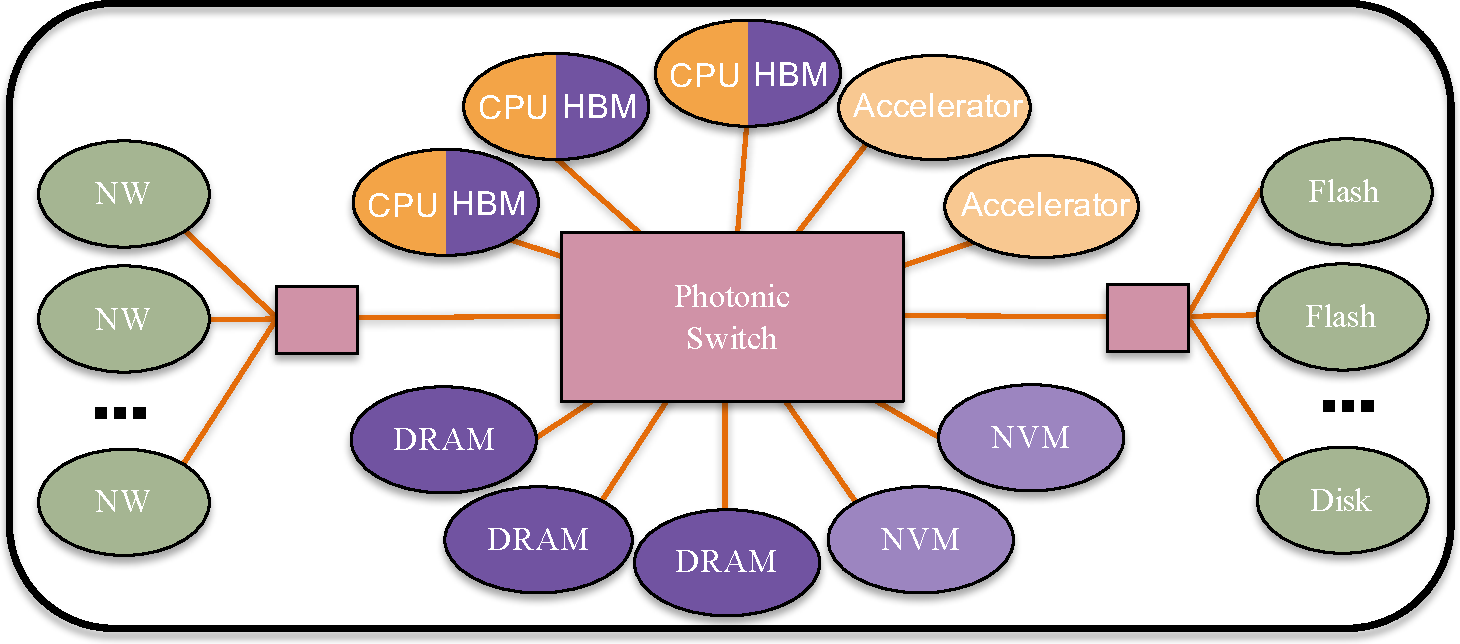
\includegraphics[width=0.9\columnwidth]{figs/FBDiagram.pdf} \label{fig:fb_diagram}
    \caption{The Firebox WSC proposal. Compute and memory resources become
    first-class citizens over a high-radix network, allowing flexible resource
    allocation and scaling. Lower-speed peripherals (such as disk or wide-area
    networking} can be connected farther away in the network topology.
\end{figure}

Firebox proposes using high-bandwidth, high-radix, networks to connect compute,
memory, and storage nodes in a \gls{wsc}. Firebox does not dictate any particular
networking technology, but is motivated by emerging integrated silicon photonic
network interfaces because they can be integrated directly on-die (or on
package, e.g., \gls{sip}), minimizing pin-out and providing high bandwidth at
low power. By multiplexing many wavelengths onto a single fiber (wave-division
multiplexing), it is possible to create a very high fanout while using few
physical interfaces. This fanout may enable very high radix switches that can
connect many SiPs within a single hop. Current estimates indicate these
photonic networks can achieve aggregate bandwidths exceeding
\SI{1}{\tera\bit\per\second} over 128 channels on a single
fiber\cite{naturePhotonic}\cite{Photonic09}. Link latencies (including photonic
transceiver crossings) are on the order of 10s of \si{\nano\second}, but final
latencies will be determined by protocol decisions. We believe round-trip
latencies (across a single switch) of approximately \SI{1}{\micro\second} to be
a conservative prediction. For reference, current infiniband EDR networks
provide approximately \SI{24}{\giga\bit\per\second} per link (with up to 12
links per NIC), and have round-trip latencies of approximately
\SI{2}{\micro\second}\cite{binnigNW}.

Compute nodes can be CPUs or special-purpose accelerators. In either case, they
will include some amount of high-bandwidth on-package memory (HBM), we
typically assume densities of approximately \SI{2}{\giga\byte} per core. This
on-package memory will have very high speed (up to
\SI{1}{\tera\byte\per\second}, at much lower power than traditional off-package
memories. A relatively large amount of on-package memory, coupled with very
fast networks allows most memory in the system to consist of network-attached memory
blades which are optimized for cost, power, and density. The total available
memory may be as much as \SI{1}{\peta\byte}. Other resources may also be used,
such as high-performance NAND flash, disks, and external network bridges.
Ultimately, the scale of such a system will be limited by network capacity, but
a Firebox would include at least thousands of cores and hundreds of
\si{\tera\byte} of bulk memory.

\paragraph{WSC Challenges}
\Glspl{wsc} promise to lower \gls{tco} significantly by improving utilization
and allowing components to develop and scale independently. These benefits
bring with them opportunities and challenges that bear mentioning. The
increased flexibility in resource allocation will require sophisticated and
scalable resource management algorithms that balance utilization, congestion,
and fairness. Encryption and authentication keys will also need to be managed
to protect memory traffic that is now exposed to attackers across the network.
In addition to being secure, memory-like interfaces must be very high
performance and any encryption or authentication mechanisms must match that
performance. Finally, this new heterogeneous memory hierarchy presents
challenges to applications and operating systems. What is the right interface
to expose the gap between local and remote memory? Will applications need to be
re-written to take advantage of it?

    \subsection{Interfaces to Remote Memory} \label{sec:rmemApproaches}
        The problem of deep and heterogeneous memory hierarchies is not entirely new;
previous mainframe and high-performance computing platforms have previously
exposed the concept of remote memory. I will describe some of these approaches
in the next two sections.

\subsubsection{Low-Level Interfaces}
\paragraph{NUMA}
\Gls{numa} architectures partition memory resources across several compute
nodes such that memory is always local to exactly one compute resource, but
still directly addressable by the others. In this case, all memory has the same
interface (loads and stores from CPUs), but some is faster than others
(non-uniform). Some \gls{numa} systems include hardware services to aid in page
migration to mitigate this effect\cite{sgi_origin}.

\Gls{numa} systems are appealing because they appear to software as a single,
large memory. They can also offer memory access latencies on the order of 100s
of nanoseconds. This performance and tight coupling, however, limit
scalability. The largest NUMA systems can scale to hundreds of nodes and 10s of
TB of memory\cite{sgiUV}, but typical systems support only a few TB and less
than 10 nodes (due to poor scaling in cost and power).

\paragraph{RDMA}
\Gls{rdma} systems are similar to NUMA in that memory resources are partitioned
among several compute nodes (memory is always local to
someone)\cite{RoCE}\cite{RFC5040}. The difference is that while NUMA systems
typically expose a cache-coherent load-store interface to both local and remote
memory resources, \gls{rdma} uses a special put/get interface to access remote
memory resources. Typically, this service is provided through the network
interface and managed by software. This interface allows RDMA systems to scale
beyond what is possible in NUMA systems, at the cost of remote memory access
performance and a more complex interface to applications.

\Gls{rdma} systems can scale to thousands of nodes and petabytes of
memory\cite{IB_ref_design}. Performance can vary, and scales with deployment
size, but modern Infiniband networks provide round-trip latencies of several
microseconds (within a rack) and bandwidths of hundreds of gigabytes per
second\cite{ib_perf}. These systems have historically been considered costly
and were primarily deployed in supercomputing environments, but recent
Ethernet-based implementations have made them increasingly
accessible\cite{RoCE}.
 
\paragraph{Memory Semantic Fabrics}
Finally, a new class of interface has been recently introduced; the
memory-semantic fabric. A memory-semantic fabric abstracts memory into a simple
load-store interface (rather than technology-specific protocols). These
interfaces are tightly coupled with the CPU, often loading memory directly into
local caches or even registers. This abstraction enables heterogeneous memory
technologies in flexible topologies. Memory thus becomes a first-class citizen
(often called a "memory blade") on a memory-optimized interconnect. The hope is
that such interfaces will allow for greater scalability and flexibility than
NUMA, while providing a more direct interface than RDMA. There are several
commercial consortia developing cache-coherent interconnects for integrating
accelerators and memories within a rack \cite{ccix}\cite{capi}. Some academic
projects have focused on scaling NUMA by increasing the level of abstraction
(e.g., \cite{sonuma}\cite{lim_disag}). Finally, an industrial effort called
Gen-Z provides a more general interface that can connect memory, accelerators,
and storage using memory-oriented operations (like load and store)\cite{genz}.
While Gen-Z does not include cache-coherence in the core specification, it can
be added through custom commands between devices that require it. It remains to
be seen how these new interconnects balance performance, scalability, and cost.

\subsubsection{Software Interfaces} The low level interfaces listed above do
not necessarily mandate a particular software interface. NUMA systems typically
expose a virtual memory abstraction to applications. In this case, the OS
manages mappings from virtual to physical addresses while hardware uses those
mappings to automatically route loads and stores to the appropriate memory
resources. The OS is also responsible for choosing which NUMA domain to
allocate memory from. This can be a complex decision and much effort has gone
into studying such allocation policies\cite{linux_numa}.

RDMA systems are further divorced from specific hardware interfaces and enjoy a
great diversity of interfaces. Some programming languages use a partitioned
global address space to make it appear as if language-level variables are all
directly accessible\cite{upc}\cite{grappa}. Other systems use RDMA more
directly to accelerate applications such as key-value
stores\cite{ramcloud}\cite{farm}.

Memory-semantic fabrics are newer and it is not clear how their interfaces
should be exposed. By coupling tightly with CPUs, it is possible to address
them directly using virtual memory. However, it may be desirable to allow
applications to choose which memory they access, or have more abstracted
interfaces (e.g., disk-like). Furthermore, these fabrics are designed to
support highly heterogeneous memory technologies. This has lead to
page-migration proposals that try to manage performance and durability
requirements either explicitly in the application, or transparently in the
OS\cite{heteros}\cite{mojim}.

In this paper, we will focus on a very general interface called demand paging
(covered in detail in the next section) that can be implemented under any of
the low-level interfaces listed here. We assume a system that allows block
reads and writes to remote memory resources. In a \gls{numa} system, this would
translate to page migration. For \gls{rdma}, we would allocate memory from
under-utilized nodes to store pages from oversubscribed nodes (as was done in
\cite{infiniswap}). In the memory-semantic approach, dedicated memory blades
would be used for remote memory and transfers would be initiated directly from
the client CPUs (e.g., using \emph{memcpy()}).

    \subsection{OS Paging Background} \label{sec:pagingBackground}
        Many architectures and operating systems expose virtual memory and paging
abstractions. While most interfaces are fairly similar, we will use the
RISC-V ISA (privileged architecture version 1.10\cite{riscv_priv110}), and
Linux version 4.15\cite{linux} for most examples in this paper.

Figure \ref{fig:generic_paging_flow} shows a typical flow for translating a
virtual address. Most translations occur completely in hardware and require no
immediate OS intervention. However, when physical memory is constrained, the
operating system may choose to store logical pages in secondary storage
(called ``paging''). This effectively treats main memory as a software-managed cache
for the storage device. In this case, some mappings are invalid (not present in
physical memory) and require immediate OS intervention (a page fault) to
resolve. Throughout this paper, we will refer to the logical data as a
``page'', and the physical location in memory as the ``page-frame'' or simply
``frame''.

\begin{figure}[h]
    \centering
    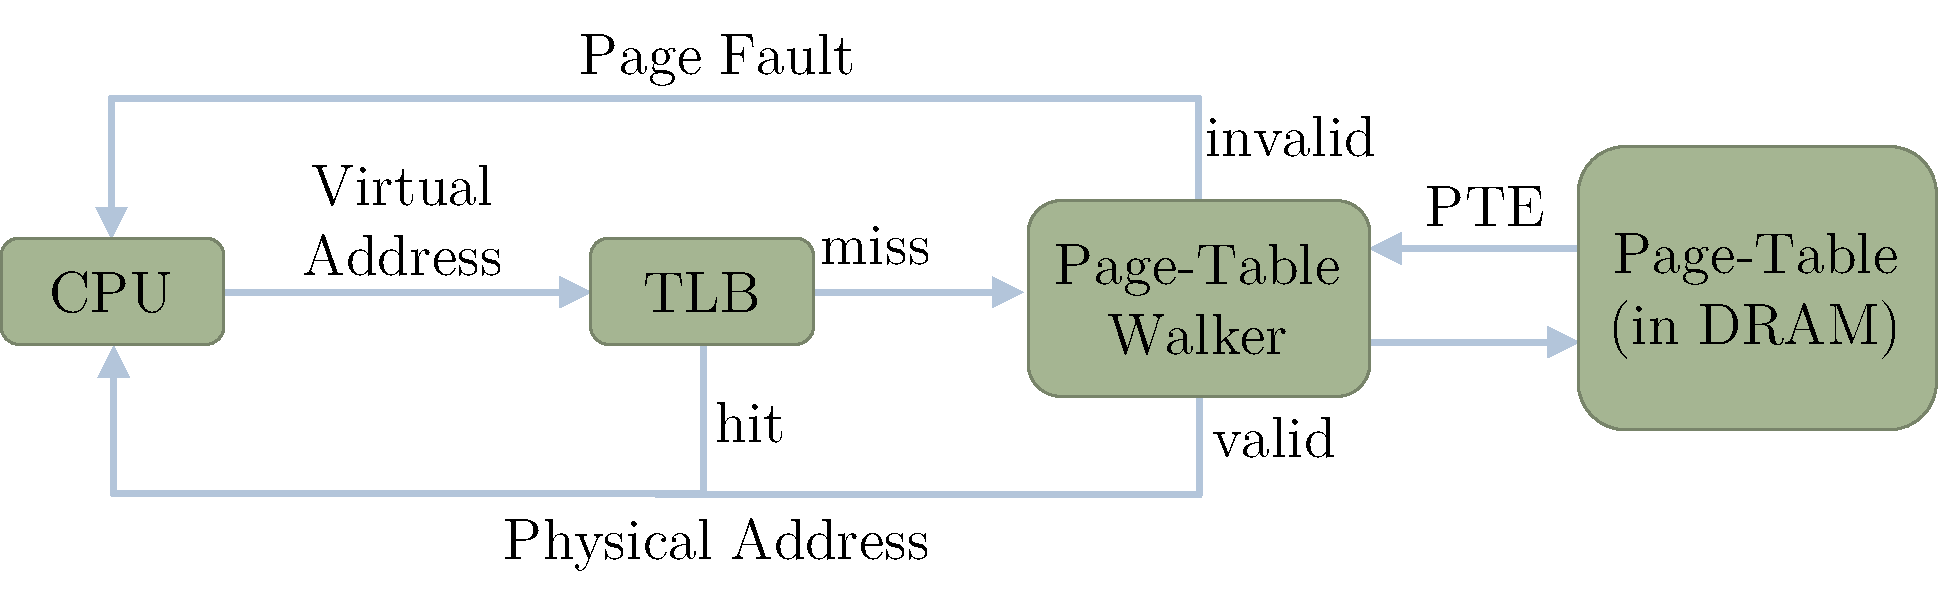
\includegraphics[width=0.9\columnwidth]{figs/generic_paging.pdf}
    \caption{Flow chart for virtual to physical address look up in a typical
      virtual memory system. The translation look aside buffer (TLB) caches
      translations. The page-table walker (PTW) fetches mappings from main
      memory when the TLB misses. Most mappings are valid and can be returned
      directly to the CPU, but invalid mappings result in a trap to the OS.}
    \label{fig:generic_paging_flow}
\end{figure}

There are three main contributors to page fault time: trap time, processing,
and backing store access. Our experiments on an Intel Haswell CPU (running at
\SI{2.6}{\giga\hertz}) show that it takes approximately \SI{800}{\nano\second}
from the time a fault occurs, to when the OS begins executing the page fault
handler. The OS then spends anywhere from \SIrange{4.5}{13}{\micro\second}
processing the fault. With backing store access times measured in milliseconds
(for e.g. a spinning hard disk), this time is insignificant. However, remote
memory systems promise access latencies on the order of several microseconds,
making page-fault processing a significant overhead.

\begin{figure}[h]
    \centering
    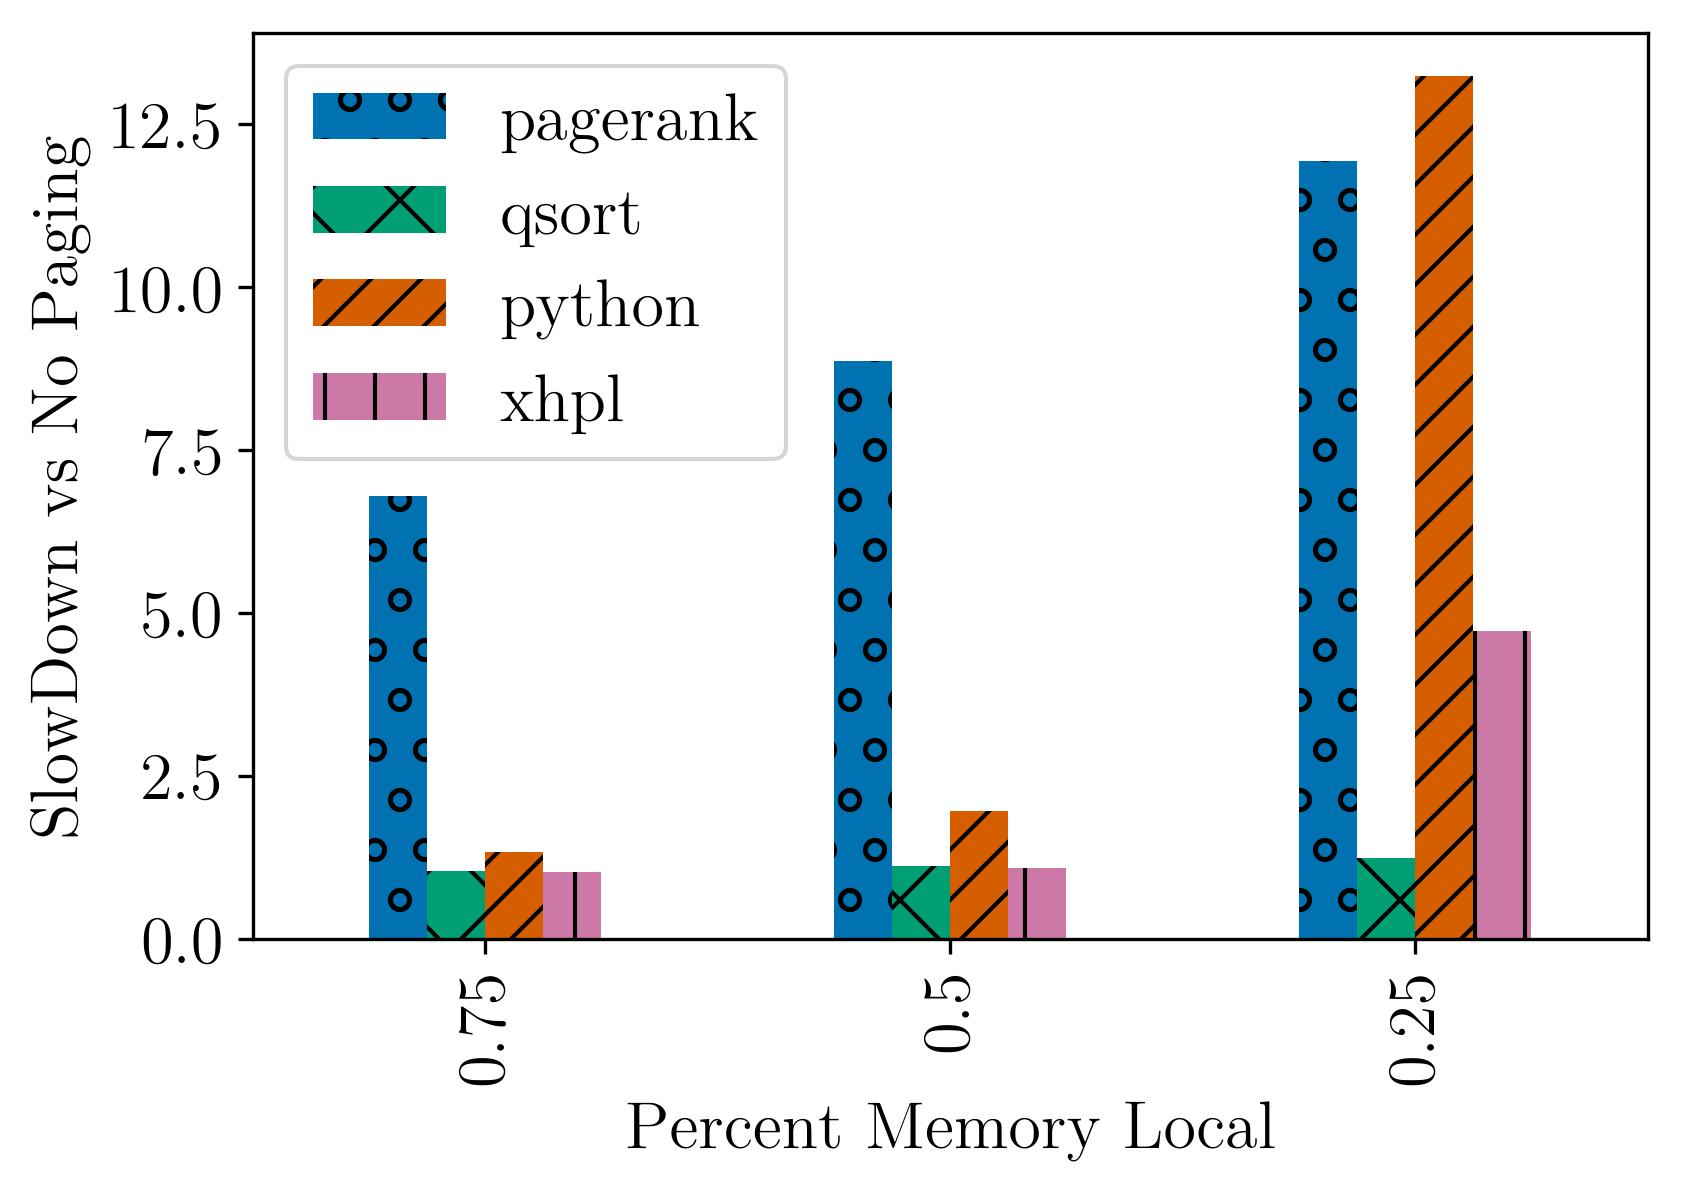
\includegraphics[width=0.9\columnwidth]{figs/paging_overhead.png}
    \caption{Application slow-down when paging to local memory. Memory
oversubscription refers to the percent of peak memory that was stored remotely.}
    \label{fig:paging_overhead}
\end{figure}

To demonstrate this, we modified the Linux kernel to swap to pre-allocated DRAM
buffers in local memory instead of an external device. This effectively
eliminates backing store access times and directly measures the overhead of
using paging at all. Figure \ref{fig:paging_overhead} plots several benchmarks'
runtime as they are run under increasingly memory constrained environments.
Note that even without waiting for secondary storage, applications can slow
down by as much as 12.5x due to paging overheads.



\section{Page Fault Accelerator} \label{sec:pfa}
    \begin{figure}[h]
    \centering
    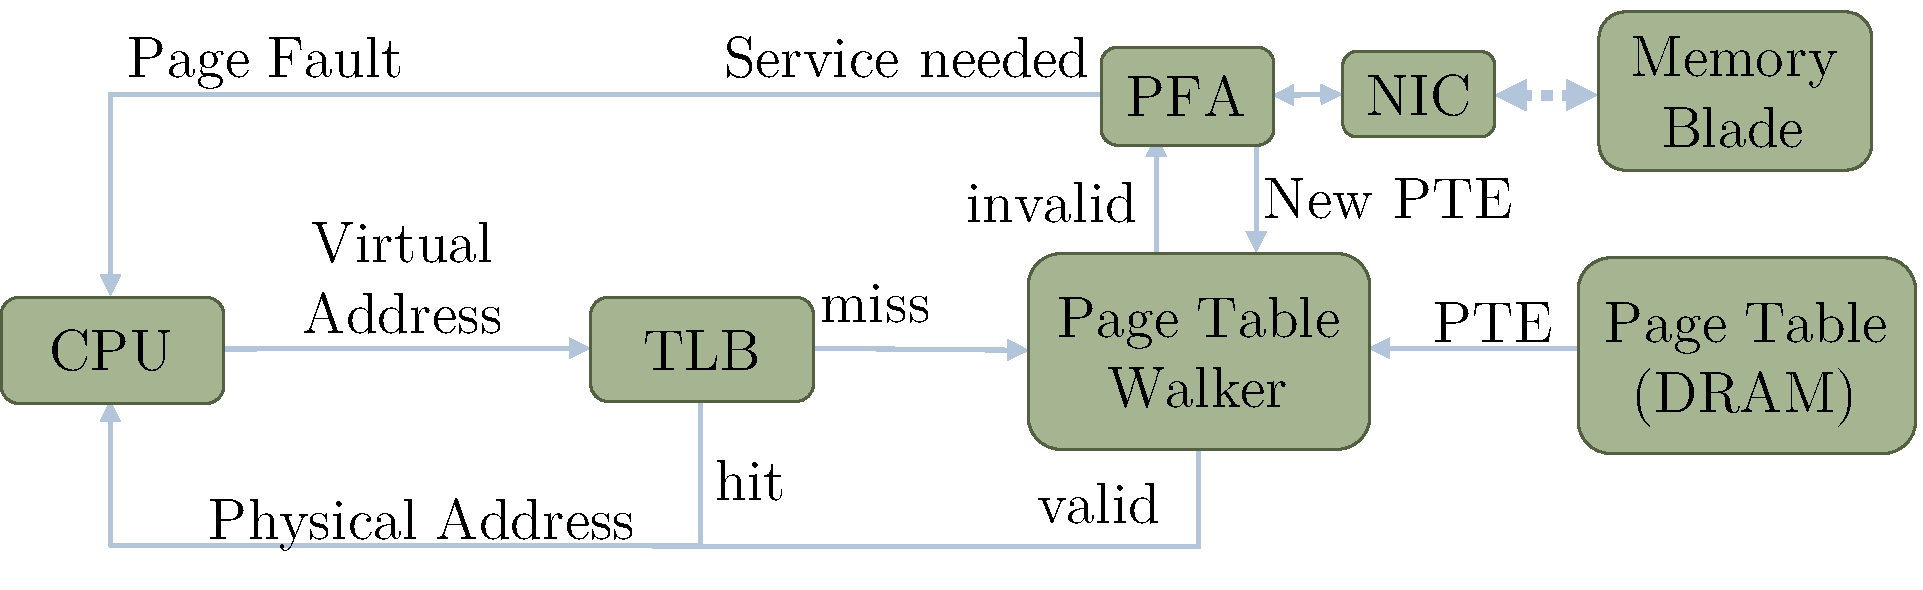
\includegraphics[width=0.9\columnwidth]{figs/generic_pfa.pdf}
    \caption{Paging with the PFA. Instead of an invalid PTE causing a trap to
    the OS (as in figure \ref{fig:generic_paging}), invalid pages are passed to
    the PFA to be fetched from remote memory. The PFA may still cause a trap if
    it cannot handle the request (e.g., full queues).}
    \label{fig:pfa_generic}
\end{figure}

Much of the work done during a page fault, while important, does not strictly
need to occur in order for the application thread to make progress. For
example, allocating free frames or updating page meta-data could be performed at
any time. Other tasks may be more efficient in hardware than in the OS; the
walking of page-tables for example. We propose a hardware accelerator that
performs only the bare-minimum of copying a remote page into a pre-allocated
frame, updating the relevant \gls{pte}, and restarting the application (figure
\ref{fig:pfa_generic}).

While this does not eliminate the need for software management of page meta-data
(here referred to as \gls{bookkeeping}), it does provide considerable flexibility
to the OS in how such \glspl{task} get scheduled. Figure
\ref{fig:bookkeeping_timeline} illustrates the difference from the perspective
of the OS. One immediate benefit is that the OS can schedule this bookkeeping
thread on idle resources, e.g. while the application is blocked on I/O.
Another benefit is that bookkeeping tasks can now be batched. Batching improves
cache locality and amortizes context switch overheads. 

\begin{figure}[h]
    \centering
    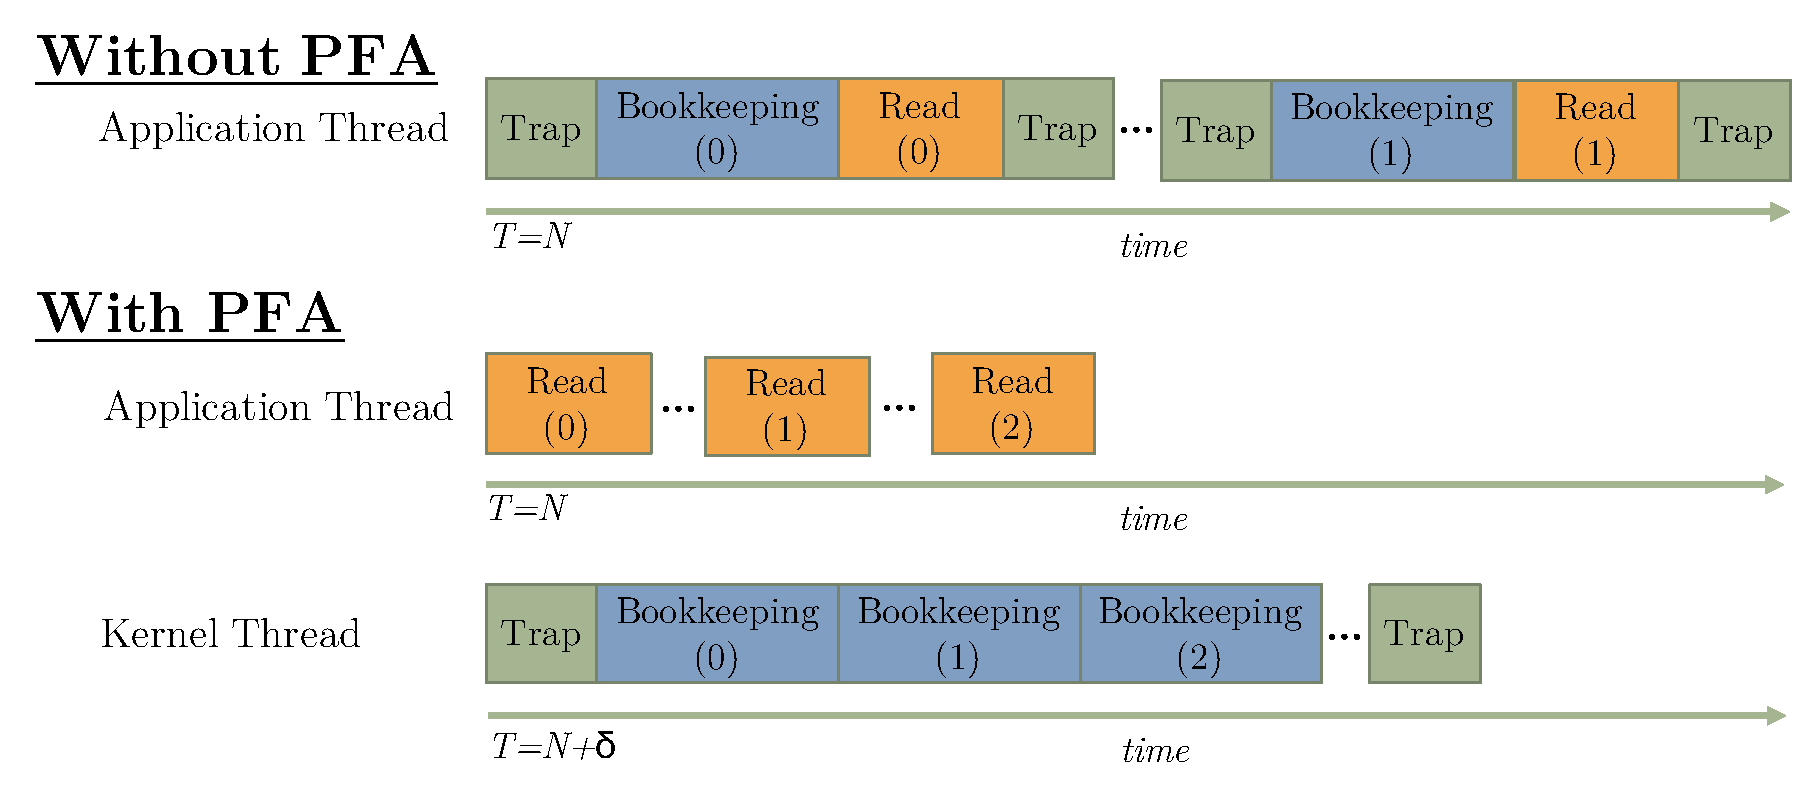
\includegraphics[width=\columnwidth]{figs/bookkeeping_timeline.pdf}
    \caption{Timeline of page-fault processing with and without the PFA.
    Without the PFA, the OS must be invoked on every page miss and perform
    various data structure look ups to decide how to handle the fault. The PFA
    allows this bookkeeping to occur any time after the fetch in a separate kernel
    thread. Only the actual page read must occur before the application can be
    restarted.}
    \label{fig:bookkeeping_timeline}
\end{figure}


    \subsection{Page Fault Accelerator Design} \label{sec:pfaDesign}
        The primary interface to the PFA is through a number of memory-mapped queues:
\gls{freeq}, \gls{newq}, and \gls{evictq}. The \gls{freeq} contains unused page
frames that the PFA can use for fetching new pages, the \gls{newq} reports any
recently fetched pages to the OS bookkeeping thread, and the \gls{evictq}
contains a list of local pages that should be stored in remote memory. Using
these queues, execution proceeds as follows:

\paragraph{Eviction}
The PFA handles all communication with the memory blade. This includes page
eviction. The basic procedure is as follows (see figure \ref{fig:evict_detail}):

\begin{outline}[enumerate]
    \1 The OS identifies pages that should be stored remotely.
    \1 It evicts them explicitly by writing to the \gls{evictq}.
    \1 The PFA sends a remote memory write command to the NIC which reads the
    page through DMA and sends it to remote memory.
    \1 When the send is complete, the PFA updates the \gls{evictq} status to
    notify the OS.
    \1 The OS stores a page identifier in the PTE and marks it as remote once
    the PFA eviction is complete.
\end{outline}

\begin{figure}[h] \centering
  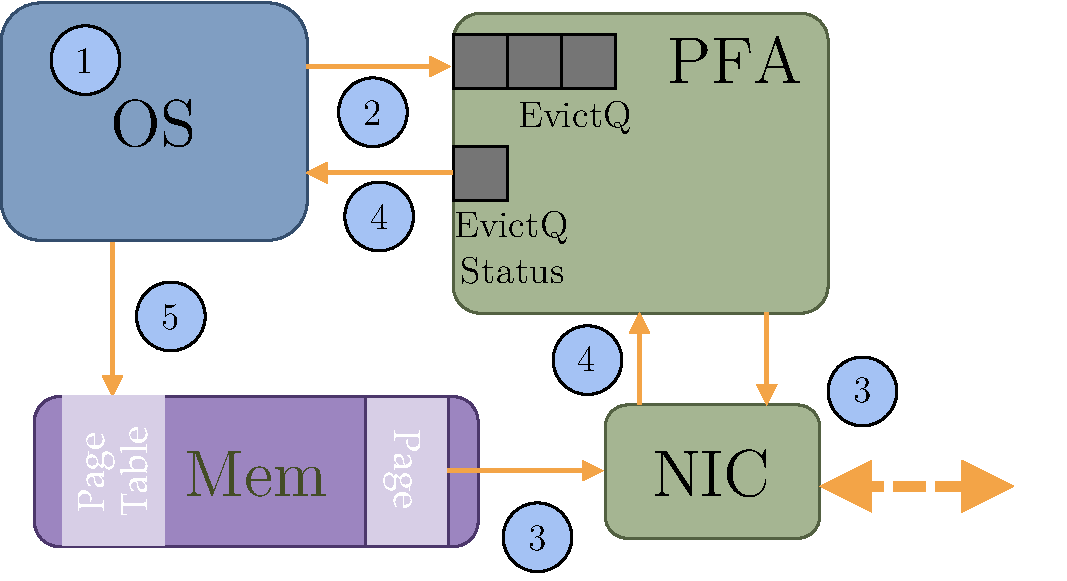
\includegraphics[width=0.7\columnwidth]{figs/pfa_evict_detail.pdf}
  \caption{Detailed eviction flow}
  \label{fig:evict_detail}
\end{figure}

In addition to the three main queues, there are a number of other maintenance
registers that are used for querying queue status and initializing the PFA. I
will mention one status register here; the EVICT\_STAT register. When a page is
placed on the evict queue, the PFA begins transferring it to remote memory, but
does not block the OS. This allows the OS to perform useful work while the
eviction is taking place, potentially hiding some of the write latency. In
order to re-use the page frame, however, the OS must poll the EVICT\_STAT
register to ensure the write has completed.

\paragraph{Fetch}
The primary function of the PFA is to automatically fetch pages from remote
memory when an application tries to access it. It does this by detecting page
table entries that are marked remote and transparently re-mapping them to the
next available free frame. The basic operation is as follows (see figure
\ref{fig:fetch_detail}):

\begin{outline}[enumerate]
    \1 Application code issues a load/store for the (now remote) page.
    \1 The TLB and PTW detect a remote page and request it from the PFA
    \1 The PFA issues a remote memory read command to the NIC, providing the
    next available frame from the \gls{freeq}.
    \1 The PFA clears the remote bit in the \gls{pte}.
    \1 The PFA pushes the virtual address of the fetched page to the NewQ.
    \1 The application is restarted.
\end{outline}

\begin{figure}[h] \centering
  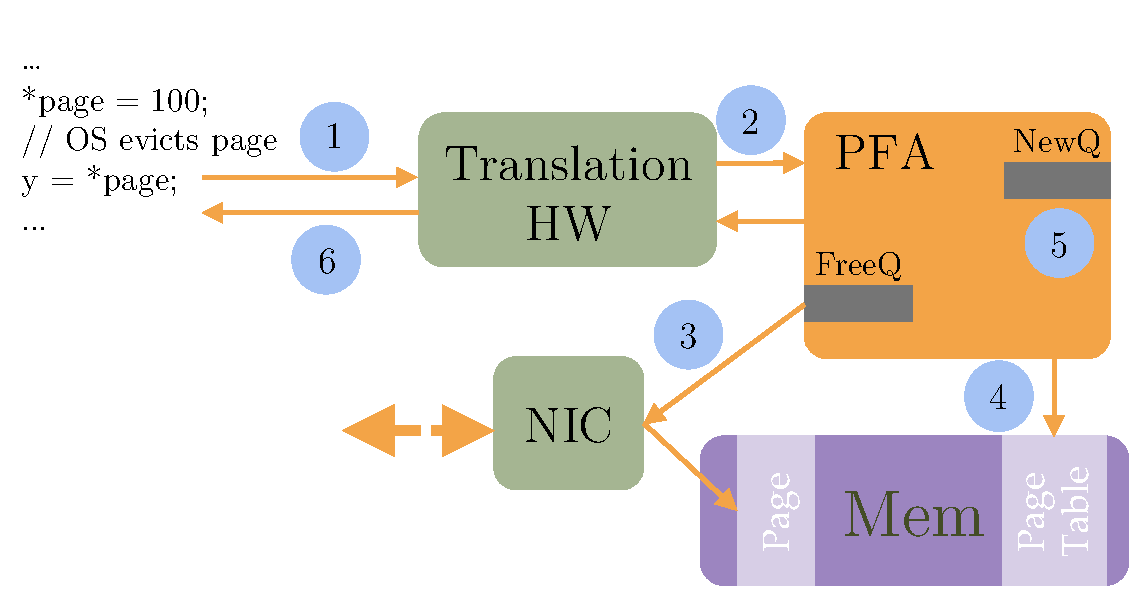
\includegraphics[width=0.8\columnwidth]{figs/pfa_fetch_detail.pdf}
  \caption{Detailed fetch flow}
  \label{fig:fetch_detail}
\end{figure}
\FloatBarrier

\paragraph{Metadata Management}
The OS should ensure that there are sufficient free frames in the \gls{freeq} to
ensure smooth operation. If a remote page is requested and there are no free
frames, the PFA will trap to the OS with a conventional page-fault. The OS must
enqueue one or more free-frames before returning from the interrupt. This may
involve evicting pages synchronously in the page-fault handler.

Similarly, the OS needs to drain the new page queue periodically to ensure it
does not overflow. This will also trap to the OS with a conventional page
fault.

% \subsubsection{Page Table Entry} \label{sec:remPTE}
% The PFA uses a special PTE format for remote pages (Figure
% \ref{fig:pte_format}). The fields are as follows:
%
% \begin{outline}
%   \1 \textbf{\gls{pgid}}: This acts as an address in remote memory for the remote
%   page. It is used by the PFA to look up pages in remote memory, and for the OS
%   to identify each page during bookkeeping.
%   \1 \textbf{Prot}: This sets the protection bits that the PFA will use when
%   fetching a page. These bits include things like read/write permissions, as
%   well as other page metadata (see the RISC-V privileged architecture manual
%   for more details \cite{riscv_priv110}).
%   \1 \textbf{R}: This bit indicates that a page is remote (when the valid bit
%   is clear).
%   \1 \textbf{V}: This indicates whether a page is valid.  A valid page is
%   currently in main memory and would not trigger a page-fault.  This is also
%   referred to as the ``present bit'' in Linux.
% \end{outline}
%
% \begin{figure}[h]
%   \centering
%   \begin{bytefield}[endianness=big,bitwidth=0.015\linewidth]{64}
%     \bitheader{0, 1, 2, 12, 40, 63} \\
%     \bitbox{24}{Unused} & \bitbox{28}{Page ID} & \bitbox{10}{Prot} &
%     \bitbox{1}{\tiny R} & \bitbox{1}{\tiny V} \\
%   \end{bytefield}
% 	\caption{Remote PTE Format. The \textbf{Page ID} is a unique identifier of this page
%   and serves as a remote memory address. The \textbf{Prot} field contains the permission
% and metadata bits that should be set after a page is fetched (see the RISC-V
% specification for details\cite{riscv_priv110}). The \textbf{R} bit indicates
% that this page is remote while the \textbf{V} bit indicates that the PTE is not
% a valid mapping (needed for backward compatibility).}
% 	\label{fig:pte_format}
% \end{figure}
%
% An interesting feature of this design is the use of pre-defined protection
% bits. This includes a valid bit which can be cleared by the OS before evicting
% to trigger a page fault on this page immediately after fetching (a useful
% debugging feature). Also, bits 8 and 9 are reserved for software by the RISC-V
% ISA and can aid the OS in bookkeeping and debugging (see Section
% \ref{sec:linuxImpl}).
%
\subsubsection{Remote Memory Interface}
The PFA requires some hardware-accessible interface to remote memory. This
could be through a memory semantic fabric or RDMA-enabled network (such as
Infiniband or RoCE). In our design, we use a custom implementation of RDMA over
ethernet to a dedicated memory blade. This interface is accessible to both
software (through a Linux driver) and the PFA (through an on-chip network).



\section{Implementation} \label{sec:impl}
    The PFA was implemented within the RISC-V ecosystem. RISC-V is an open-source
instruction set with several open and closed-source implementations and ports
for many common software components\cite{riscv}.

% \subsection{PFA Reference Implementation}
% To accelerate software development, and to provide a golden-model of
% PFA behavior, we implemented the PFA first in a RISC-V ISA simulator called
% "Spike"\cite{spike}. Spike provides a functional simulation of a RISC-V core
% through a straightforward C++ interpreter, but does not provide any timing
% accuracy. Due to its simplicity, the PFA implementation required only a few
% weeks of implementation effort and less than 1000 LoC. With Spike, software
% development was able to proceed concurrently with the concrete hardware design.
% Furthermore, unit tests developed under Spike were used to validate the
% hardware implementation, reducing debugging effort. In all, the only software
% change that was needed to go from Spike to a concrete implementation was one
% extra TLB flush due to a difference in TLB design between Spike and the RISC-V
% implementation we used.
%
\subsection{Hardware Implementation}
The PFA prototype was implemented in the Chisel hardware construction
language\cite{chisel} and integrated with a simple in-order CPU called
RocketCore\cite{rocketchip}. The components were integrated using the
RocketChip system-on-chip (SoC) generator\cite{rocketchip}. We provide an
overview of the relevant systems in the following sections. The current PFA
prototype implements a subset of the specification described in Section
\ref{sec:pfaDesign}. Specifically, it does not support multiple simultaneous
evictions (the EvictQ has an effective depth of 1), however, it does allow for
asynchronous eviction. This prevents optimizations such as switching to other
threads while many pages are simultaneously evicted (a single eviction does not
take long enough to justify a context switch). 

\subsubsection{RocketCore and RocketChip}
RocketChip\cite{rocketchip} is a framework for generating SoCs. It includes
on-chip interconnects, caches, and other utilities for chip construction. While
the CPU is pluggable, we use only a single RocketCore in-order CPU for our
experiments. Our implementation used dedicated 16KB instruction and data
caches \todo{Details of rocket target}. While the node had access to several gigabytes of main memory, we
artificially limited application memory using Linux cgroups (see Section
\ref{sec:eval} for details). A real \gls{wsc} would likely include a mixture of
simple cores, high single-thread performance cores, and
accelerators. We hope to evaluate the Berkeley out-of-order core
(BOOM\cite{BOOM}) and the Hwatcha vector accelerator\cite{hwatcha} in the
future when they become available in our simulation infrastructure.

\subsubsection{FireSim}
We simulated the RTL using a cycle-accurate simulator called
"FireSim"\cite{firesim}. FireSim is an FPGA-accelerated simulator that runs on
the Amazon cloud. It can simulate thousands of nodes with a cycle-accurate
network and heterogeneous components. Many parameters of the simulation are
tunable within FireSim. We decided on a \SI{200}{\giga\bit\per\second} network
with \SI{500}{\nano\second} link latency, leading to roughly 2us page access
time to the memory blade (similar to current infiniband networks).

\begin{figure}[h]
\centering
\begin{tabular}{| l | l |}
  \hline
  \textbf{CPU Type} & Rocket (5-stage in order) \\ \hline
  \textbf{CPU Frequency} & \SI{3.2}{\giga\hertz} \\ \hline
  \textbf{Caches} & \SI{16}{\kilo\byte} D\$ and I\$ \\ \hline
  \textbf{NW Topology} & Single Switch \\ \hline
  \textbf{NW Bandwidth} & \SI{200}{\giga\bit\per\second} \\ \hline
  \textbf{NW Link Latency} & \SI{2}{\micro\second} \\ \hline
  \textbf{Remote Page Read} & \SI{4.8}{\micro\second} \\ \hline
  \textbf{Remote Page Write} & \SI{4.8}{\micro\second} \\ \hline
\end{tabular}
\caption{System parameters used for evaluation.}
\label{tbl:sim_parameters}
\end{figure}

\subsection{Linux Integration} \label{sec:linuxImpl}
    We modified the Linux kernel (version 4.15\cite{linux}) to support the PFA. The
majority of software development was done using the functional simulator.

% \subsubsection{Non-PFA Paging in Linux} \label{sec:vanillaLinux}
% We will now briefly describe how paging works in vanilla Linux. Note that the
% kernel internally uses the term \gls{swap} in reference to all paging activity,
% we will use these terms interchangeably. For a more complete discussion of
% memory management in Linux, see \cite{linuxBook}. Figures
% \ref{fig:vanilla_evict} and \ref{fig:vanilla_fetch} map out the steps involved
% in evicting and fetching pages, respectively.
%
% \paragraph{Page Reclaiming}
% Linux manages memory limits on a per-task basis. In this case, a \gls{task}
% refers to the kernel-specific abstraction of a process. Each task has its own
% resource limits which are exposed to system administrators through the
% \gls{cgroup} interface. When a task approaches its assigned limit of a certain
% resource, it is throttled in a resource-specific manner. In the case of memory,
% the kernel attempts to free task-assigned memory. It will first attempt to
% shrink any file caches (especially clean disk blocks that can simply be deleted
% without requiring any disk activity). If shrinking caches is not enough, the
% kernel begins to page non-file backed pages (called ``\glspl{anonpg}''). This
% is done using a pseudo-\gls{lru} eviction algorithm (Step 2 in Figure
% \ref{fig:vanilla_evict}). Page reclaiming can be triggered
% in one of two ways (Step 1). If a hard memory limit is met, but more memory is needed to
% proceed, then page-reclaiming happens synchronously (called direct reclaim).
% However, Linux tries to avoid this scenario by running a background thread
% called \gls{kswapd} that begins reclaiming pages when the application reaches a
% soft resource limit. \Gls{kswapd} is usually idle, but can be woken up when the
% kernel detects a soft limit has been met. It also runs with a low priority to
% avoid wasting resources on speculative evictions (the application may never hit
% its hard limit).
%
% \begin{figure}[h] \centering
%   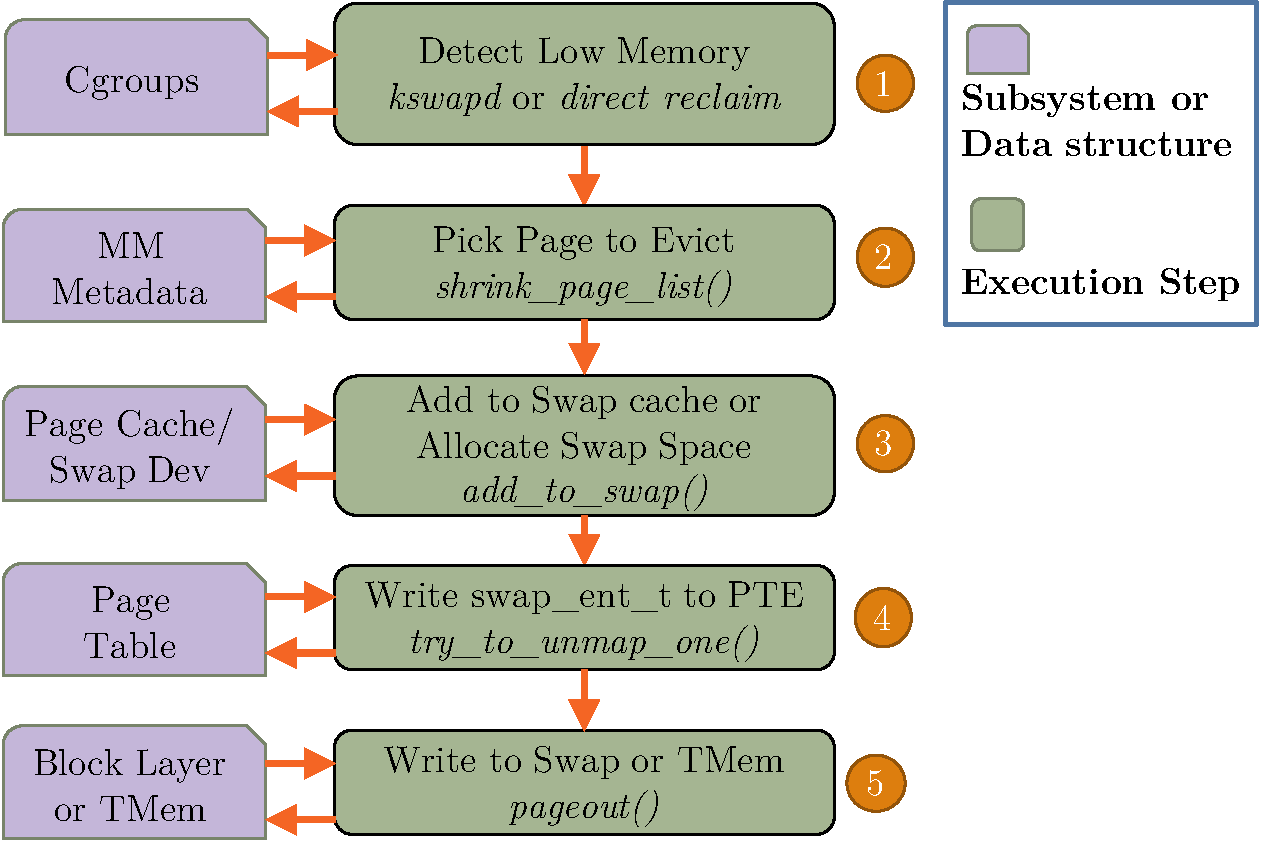
\includegraphics[width=0.9\columnwidth]{vanilla_evict.pdf}
%   \caption{Baseline Linux page eviction (reclaim) code path.}
%   \label{fig:vanilla_evict}
% \end{figure}
%
% \paragraph{Page Eviction}
% Paging was originally intended to use hard disks as the backing store, and this is
% reflected in the design of paging in Linux. To swap, one or more block
% devices must be formatted and mounted as swap devices. Linux then uses the
% block offset on this disk as a unique identifier for an evicted page (Step 3). In
% order to support more complex paging schemes (such as page compression, or
% heterogeneous memory), Linux introduced the \gls{tmem} layer\cite{tmem}. This
% scheme still uses disk offsets as identifiers, but completely bypasses the block
% layer. This is important because many optimizations in the block layer (e.g.,
% write coalescing and block reordering) are not suitable for these alternative
% paging devices. Evictions do not immediately result in writes to \gls{tmem} or
% a swap device. Instead, pages are stored in a data structure called the swap
% cache (Step 3). This swap cache helps reference count shared pages, and hedges
% against poor eviction choices. Once a page is no longer physically available,
% Linux replaces the corresponding \gls{pte} with a \gls{swpent} which clears the
% valid bit, and uses the remaining bits to store the swap device ID (called
% ``type'' in the kernel) and block ID (called ``offset'') (Step 4).  When
% changing a \glspl{pte}, most architectures require the OS to flush the
% \gls{tlb}. This forces a page-table walk on the next access to this virtual
% address. Finally, the kernel begins a write to the swap device in the
% background (Step 5).
%
% \paragraph{Page Fetch}
%
% \begin{figure}[h] \centering
%   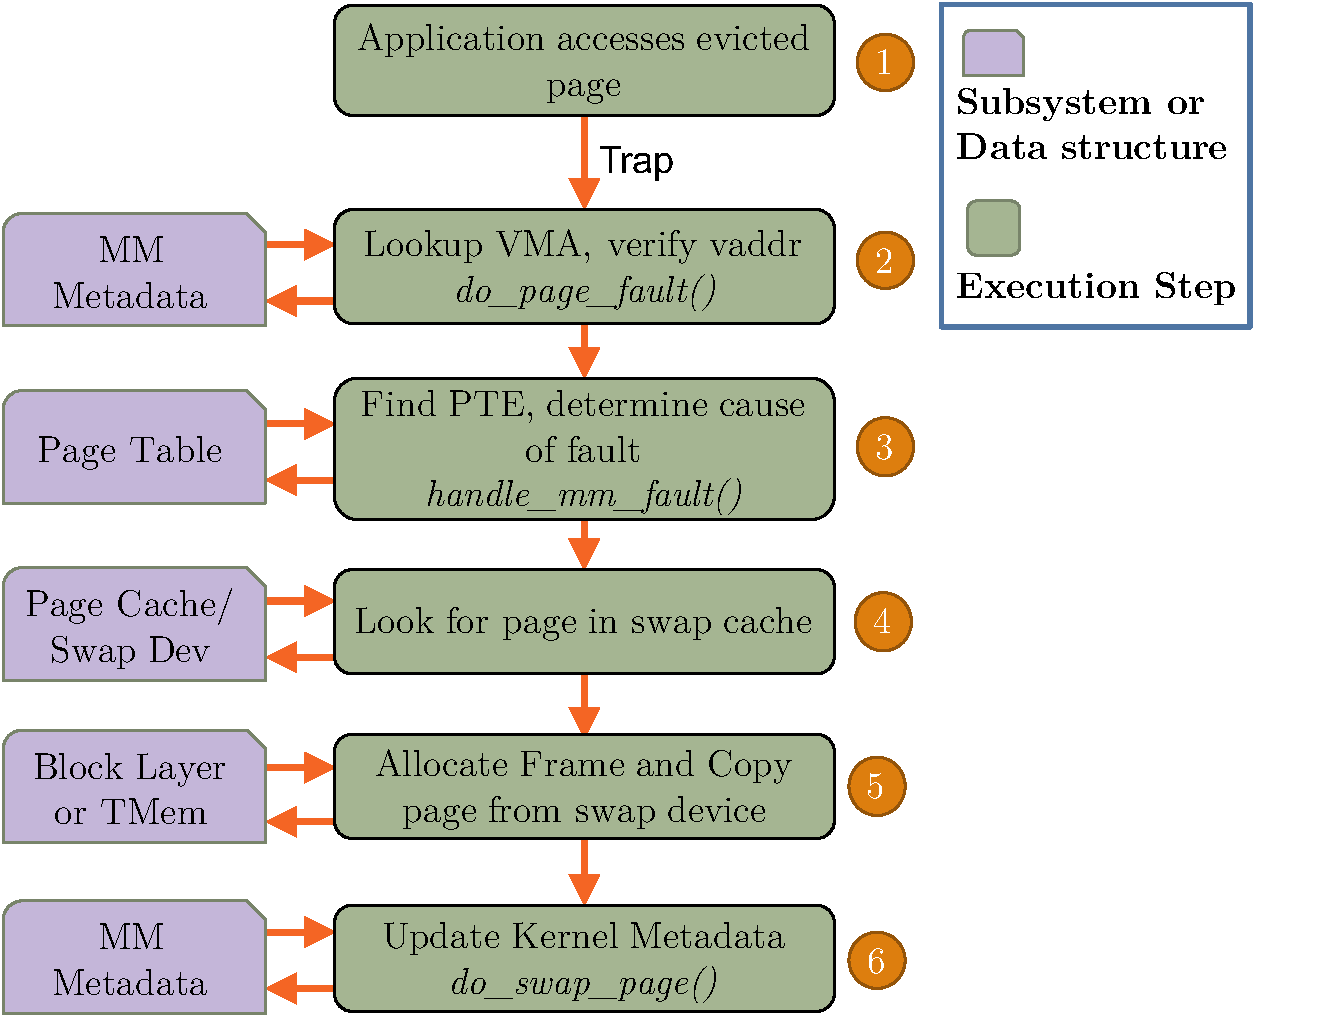
\includegraphics[width=0.9\columnwidth]{vanilla_fetch.pdf}
%   \caption{Baseline Linux page fetch code path.}
%   \label{fig:vanilla_fetch}
% \end{figure}
%
% When a user program attempts to access a page that has been swapped out, the
% \gls{ptw} notices the invalid PTE and issues a page fault trap to the OS (Step
% 1 in Figure \ref{fig:vanilla_fetch}). Note that hardware does not examine
% the remaining bits (the \gls{swpent} is purely a software construct). Upon
% receiving a page fault, Linux first determines if the requested virtual address
% has been assigned to this task. It does this by iterating through regions of
% virtual memory called \glspl{vma} (Step 2). If a valid \gls{vma} is found, then
% the OS begins a \gls{pgtbl} walk to locate the corresponding \gls{pte}. There
% are several reasons that a page fault may occur, the OS must check the
% \gls{pte} to determine the cause (Step 3). Assuming the cause was an invalid
% \gls{pte}, the OS then searches the swap cache for this page (Step 4). This is
% in case some other process that shares it has already brought it in. If the
% page is not found, then a new frame is allocated and a transfer is initiated to
% read the page from the swap device (Step 5). If the page is found in
% \gls{tmem}, then the transfer occurs synchronously, otherwise the process
% initiates the transfer and then yields to the scheduler, resulting in a context
% switch. When the transfer is complete, the kernel changes the PTE from a
% \gls{swpent} to a valid PTE with permissions defined by the \gls{vma}. Finally,
% the kernel updates page-tracking meta-data (Step 6). This includes the \gls{lru} lists
% maintained by the eviction algorithm, \gls{vma} membership, and a number of
% other kernel subsystems. Note that several of these updates require
% synchronization with other kernel threads. Once all bookkeeping is complete,
% and the PTE is updated, the kernel flushes the \gls{tlb}, and restarts the
% application.

\subsubsection{PFA Modifications}
The introduction of a PFA changes a number of the assumptions underlying
baseline paging behavior. Figure \ref{fig:linux_changes} summarizes these
changes.

\begin{figure}[h] \centering
  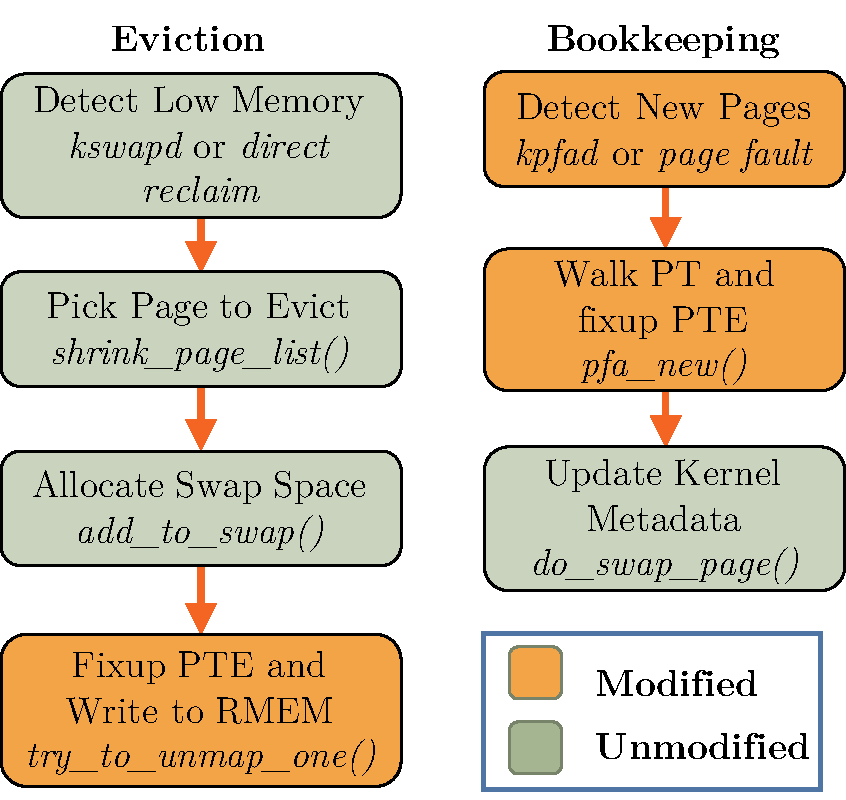
\includegraphics[width=0.7\columnwidth]{linux_changes.pdf}
  \caption{Major changes to Linux paging to accommodate the PFA. Most
  subsystems could be re-used without change. On the eviction path, all that
  was changed was the PTE update (to write a remote \gls{pte} instead of a
  \gls{swpent}), and the write to disk (to write to remote memory instead). The
  bookkeeping path is now triggered either from the page-fault handler (due to
  a PFA service request) or from \gls{kpfad}. The core bookkeeping function
remains unmodified.}
  \label{fig:linux_changes}
\end{figure}

% \paragraph{Frame Allocation and Permissions}
% Linux uses the faulting virtual address to make a number of decisions during
% the page fetch process. For instance, the permission bits are taken from the
% \gls{vma}. \gls{vma} information is also used to decide which physical frame to
% use (this is particularly important in NUMA systems). With the PFA, however,
% the OS must decide on this information at \emph{eviction} time. Pre-allocating
% physical frames is not an issue in our system because there is only one core,
% and frame selection does not depend on the \gls{vma}. Permission bit selection
% is more problematic. Our current approach is to assign permission bits to a
% remote page based on the \gls{vma} permissions at the time of eviction, we then
% update those permissions while performing bookkeeping. In practice, this is
% unlikely to cause problems as permissions rarely change. Furthermore, Linux is
% able to correct inappropriately restrictive permissions during page-faults.
% However, there may be security concerns if permissions are made more
% restrictive while a page is remote. This vulnerability exists in the window
% between page fetch and bookkeeping. To mitigate this concern, the OS would need
% to be modified to update remote PTEs when changing \gls{vma} permissions.
%
% Under these simplifying assumptions, we are able to allocate frames
% proactively. The current implementation always refills the \gls{freeq} during
% bookkeeping. To simplify the bookkeeping procedure, we track
% each allocated frame in a FIFO queue. This allows the bookkeeping code to simply pop
% this queue to find which frame was used for each new page (the PFA always drains
% the \gls{freeq} in FIFO order).

% \paragraph{Asynchronous Bookkeeping}
% In normal paging, the \emph{do\_swap\_page()} function is able to update meta-data as
% soon as a page is fetched. With the PFA, we delay this bookkeeping for a
% bounded but potentially non-trivial period of time. Many of these bookkeeping
% tasks are in support of heuristics or resource accounting (e.g., LRU lists for
% eviction, or memory utilization metrics). Delaying these tasks reduces the
% accuracy of various algorithms, but does not result in incorrect behavior.
% Others are needed for correct execution (e.g., \gls{vma} membership or shared
% page tracking for copy-on-write). We address these correctness issues by
% performing bookkeeping preemptively before accessing any of the related
% algorithms. These tasks may be fairly common, but they are unlikely to actually
% involve a recently fetched page. To avoid preemptively performing bookkeeping,
% we use one of the reserved bits in the PTE protection field to indicate a page
% that has been recently fetched but not yet processed. This bit gets set at
% eviction time, but is cleared during bookkeeping.
%
% \paragraph{Swap Device and Block ID Allocation}
% Linux assumes that all swap activity is backed by a block device and it uses
% the physical address on this device to identify all evicted pages. This block
% ID is needed during the bookkeeping process to identify the page. To address
% this problem we make a number of simplifying assumptions.
%
% \begin{outline}[enumerate]
% 	\1 \textbf{A real swap device is available} (even though it is not used). We
% 		use a ram-based file system (ramfs) to trick the kernel into thinking it has
% 		a large disk attached. This uses no actual physical memory.
% 	\1 \textbf{There is only one swap device.} This allows us to not track device
% 		ID. This is achieved by making the ramfs sufficiently large to address all
% 		swap activity.
% 	\1 \textbf{Block IDs are contiguous on the integers $\mathbf{(0, 2^{28}]}$.}
% 		This allows us to pack the block ID into the remote PTE format (see Section
% 		\ref{sec:remPTE}). We achieve this by ensuring that the ramfs is the same
% 		size as our memory blade (and less than $2^{28}$ pages). Since block IDs
% 		correspond to physical offsets on the swap device, we are guaranteed to
% 		never see an invalid block ID.
% \end{outline}
%
% While these assumptions hold, we are able to compress the \gls{swpent} into a
% \SI{28}{\bit} PageID by eliding the type, and using the offset directly.
% Finally, we avoid overheads in the block layer by implementing the PFA as a
% \gls{tmem} device. Since bookkeeping is asynchronous, and eviction occurs
% earlier in the process (due to ordering constraints with PTE modifications),
% this \gls{tmem} plugin simply returns immediately. The current implementation
% evicts synchronously. This is because the expected write time is much smaller
% than a scheduling quantum and asynchronous eviction would result in wasteful
% context switches. Future implementations may attempt to overlap eviction with
% low-latency tasks such as bookkeeping.
%
\subsubsection{kpfad} \label{sec:kpfad}
The most basic implementation of PFA support in Linux simply performs
bookkeeping tasks whenever the internal queues of the PFA fill up. This
effectively batches page bookkeeping, but it does not allow the kernel to
choose when the bookkeeping occurs. To leverage idle periods in
program execution, or unused hardware threads, we implement a background
bookkeeping daemon called \gls{kpfad}. \Gls{kpfad} is triggered by an adaptive
timer that attempts to discover the average time between full queues. It does
this by increasing the wait time by a small amount every time it runs, and
decreasing the time whenever the application is interrupted due to full queues. 
While \gls{kpfad} gives increased flexibility and efficiency on a lightly
loaded system, it causes strictly more overhead than interrupt-driven
bookkeeping when the application has enough work to keep all hardware threads
busy (since the adaptive timer is not perfect). To avoid this, \gls{kpfad} is run
with very low priority (similar to the page-out daemon \gls{kswapd}). Unlike
\gls{kswapd}, however, \gls{kpfad} does not get triggered by a soft limit. We expect
the adaptive timer scheme, coupled with low priority, to be sufficient to avoid
significant overhead.

\subsubsection{Baseline Swapping}
We modified Linux to use the remote memory blade while paging. This was done by
implementing a software interface to the remote memory blade as a \gls{tmem}
device. The swapping mechanism uses a custom NIC driver that provides zero-copy
semantics and bypasses the normal Linux networking stack. 




\section{Evaluation} \label{sec:eval}
    \subsection{Experimental Design} \label{sec:expDesign}
  Our evaluation is based on two benchmarks with significantly different access
  patterns. The first is quicksort (Qsort). This benchmark first allocates a
  large array of random numbers, and then sorts it using the well-known
  quicksort algorithm.  Quicksort is a divide and conquer algorithm that
  automatically partitions the input array into small local blocks before
  performing a final sort. This leads to excellent cache behavior and
  predictable access patterns.  Furthermore, by allocating the input array
  dynamically, quicksort performs no file I/O, so it is never blocked on I/O or
  other OS interactions.

  The other benchmark is a de-novo genome assembly benchmark (Gen). Gen begins
  by loading a large text file that represents raw genome data. Raw genome data
  consists of short, overlapping, sequences of base-pairs called "contigs", the
  goal is to align these overlapping contigs into a single contiguous sequence
  representing a genome. This is done by loading contigs into a large hash
  table and probing into it repeatedly to find matching sequences. This leads
  to very little locality and unpredictable access patterns. Furthermore, Gen
  performs file I/O on the input, which allows for more complex OS
  interactions.
\newline
\newline
  \begin{lstlisting}[frame=single]
# Data Schema
result = NamedTuple(
	'mean', # Mean results from 10 runs
	'std', # Standard deviation from 10 runs
)

# mean and std have the same set of keys
result.mean.keys
[ 't_run', 't_bookkeeping', 't_rmem_write',
  't_rmem_read', 'n_fault', 't_fault',
	'n_swapfault', 'n_pfa_fault', 'n_early_newq',
	'n_evicted', 'n_fetched', 'n_kpfad',
	't_kpfad', 'slowdown']

# Datasets
# Paging to remote memory in SW ('baseline')
base_res = ingest_run('raw/results_baseline.csv', 'rv')

# Paging using the PFA to real memblade
pfa_res = ingest_run('raw/results_pfa.csv', 'rv')

  \end{lstlisting}

\subsection{End-to-End Performance} \label{sec:fullPerf}
  The benchmarks were both run under a cgroup in Linux in order to reduce the
  available memory and emulate a system where applications would need to share
  limited local memory. This is the same mechanism that system administrators
  use today to control application memory consumption (e.g., in containers). In
  this experiment, we disable kpfad in order to isolate the batching of
  new-page management from the scheduling flexibility offered by kswapd's
  asynchrony.  The PFA was configured to allow up to 64 outstanding page faults
  before bookkeeping was performed.
  \newline
  \newline
  \lstinputlisting[frame=single]{real-pfa.patch}

  Both applications use 64MB of memory at their peak. We then
  varied the cgroup memory limit from 100\% (64MB) down to 25\% (16MB),
  triggering increasing levels of paging. For both benchmarks, the PFA reduces
  end to end run time by up to 1.4x.

  \begin{figure}[bht] \centering
    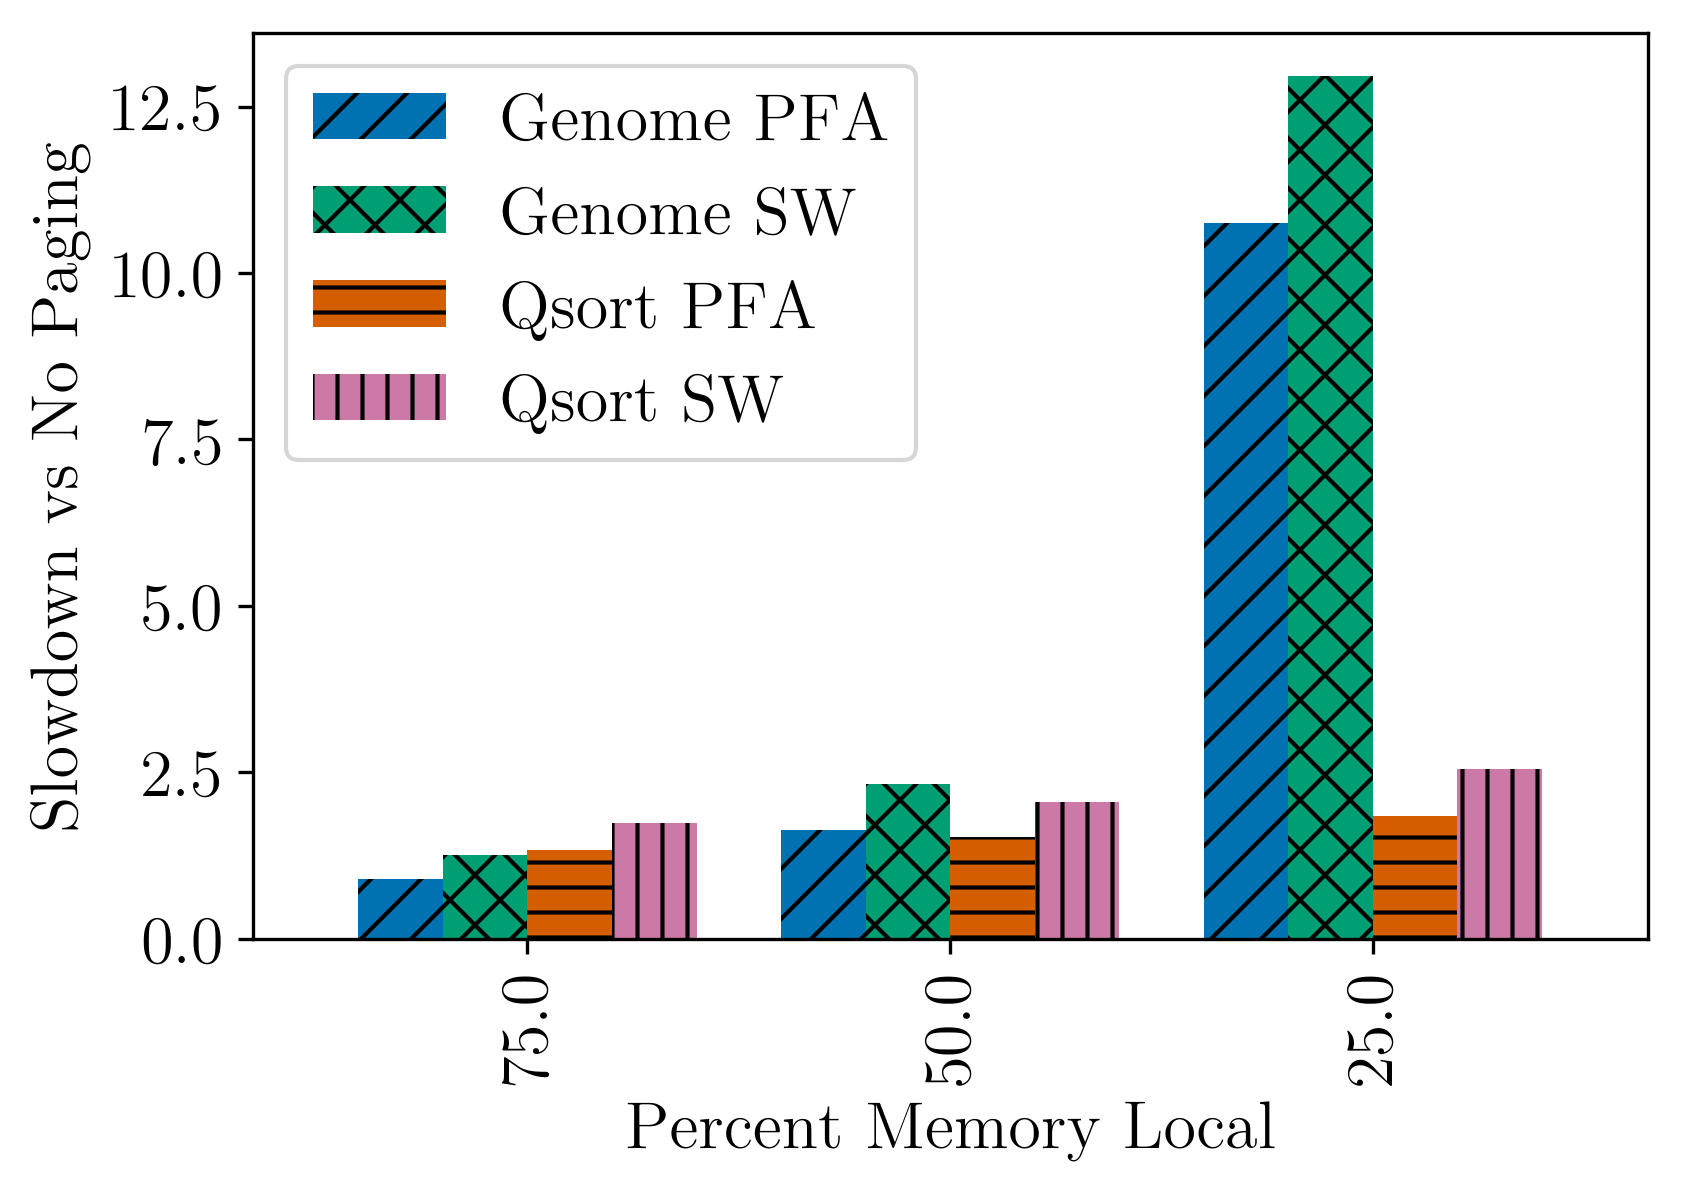
\includegraphics[width=0.5\columnwidth]{figs/perf_nokswapd.png}
    \vspace{+1cm}
    \caption{PFA vs Baseline without kswapd. Applications run approximately
    20-40\% faster when the PFA is enabled.}
    \label{fig:pfa_perf}
  \end{figure}

\subsubsection{Analysis}
  We now analyze the sources of this performance improvement.

  \paragraph{Fetch Times}
  We begin our analysis by looking at the key metric of average fetch time.
  This is the time between when an application attempts to access a remote
  page, and when it is able to continue processing. In this experiment, we use
  a simplified memory blade and network implementation with a constant
  \SI{4}{\micro\second} access latency in order to better understand local
  overheads. Figure \ref{fig:fetch_breakdown} plots the time for accessing a
  single remote page on an unloaded system. We classify time into four
  categories:

  \begin{outline}
    \1 \textbf{Trap:} The time for the hardware to detect an invalid access and
    context switch to the OS.
    \1 \textbf{Proc:} The time spent processing the page locally (overhead).
    \1 \textbf{NIC:} The time spent interacting with the network interface.
    \1 \textbf{MemBlade:} The time spent on the network and in the memory
    blade.
  \end{outline}

  Recall from Section \ref{sec:pfa} (and Figure \ref{fig:bookkeeping_timeline}
  in particular) that the PFA moves some of this processing (especially
  \textbf{Proc}) to an independent kernel thread; we account for this in a
  later section. 

  \begin{figure}[h] \centering
    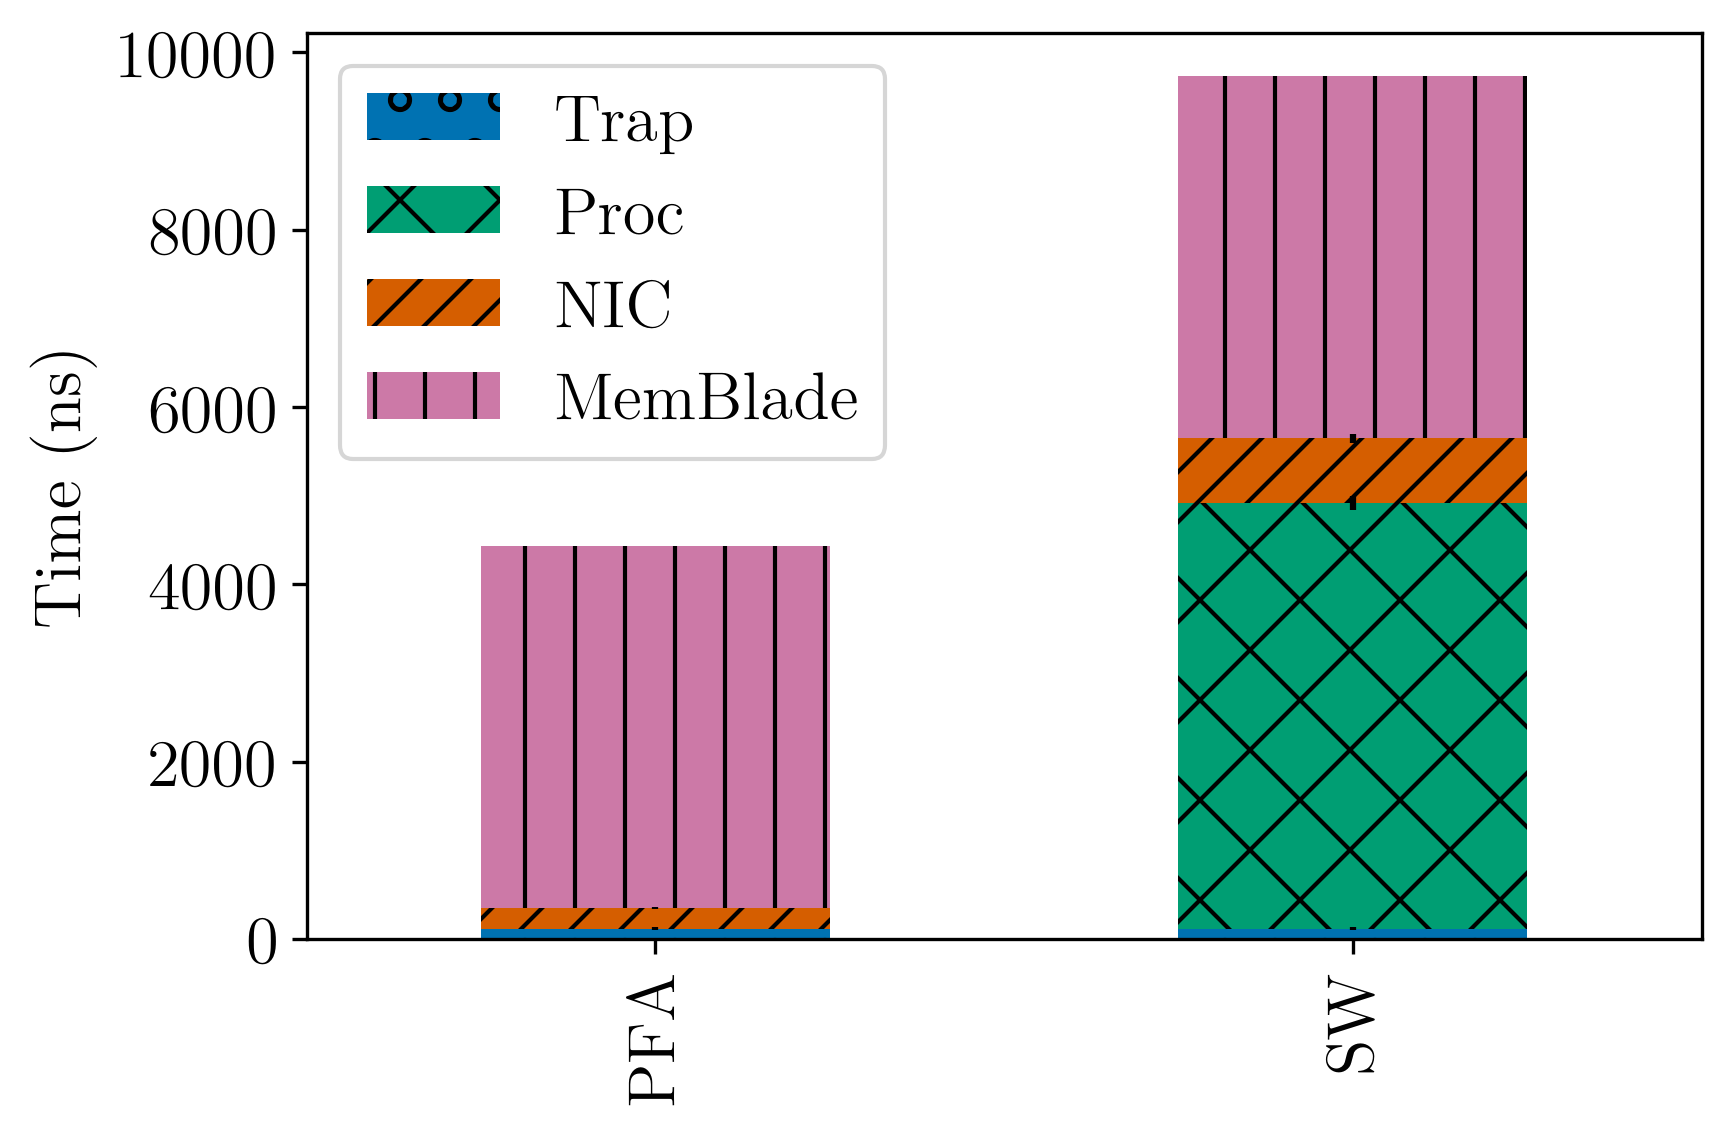
\includegraphics[width=0.8\columnwidth]{figs/fetch_breakdown.png}
    \caption{Breakdown of time in fetching a single remote page. All data are 
    the average of 10 runs. Error bars represent standard deviation (but are
  almost too small to be seen). Note that local processing time (including
  the trap and NIC interaction) only accounts for 8\% of time with the PFA, but
  accounts for over 50\% of time for the baseline.}
    \label{fig:fetch_breakdown}
  \end{figure}

  Note that the trap overhead is a very small fraction of total time (just
  \SI{113}{\nano\second}). This is a result of using a simple in-order RISC
  core like Rocket. It is likely that this overhead may be more significant on
  a more complex architecture like server-grade x86 cores. Next, note that the
  time spent on the network and in the memory blade accounts for less than half
  the time in the baseline implementation, but completely dominates the PFA
  fetch time. This effect will be even more pronounced as network and memory
  blade performance improves. For example, if \textbf{MemBlade} time were
  reduced to \SI{1129}{\nano\second} to simulate a \SI{1}{\tera\bit\per\second}
  link with \SI{1}{\micro\second} round-trip latency (as predicted in Section
  \ref{sec:firebox} for photonic networks), then client-side processing would
  account for 83\% of time in SW but only 23\% of time with the PFA. Finally,
  note that the \textbf{NIC} time in software is larger than the total time in
  the PFA. We believe this is due to a more efficient hardware to hardware
  interface between the PFA and the NIC. While not visible in the figure, the
  actual PFA-specific processing takes only 1 cycle in hardware, the remaining
  time is split between detecting and delivering the remote PTE to the PFA
  (\textbf{Trap}), and interacting with the NIC (\textbf{NIC}). The total time
  to fetch a page with the PFA is 2.2 times faster than in SW, but this does
  not tell the whole story; The PFA does not eliminate the work that is done
  during SW \textbf{Proc}, it simply moves it to another thread. Likewise, the
  \SI{113}{\nano\second} trap overhead may seem small, but this does not
  account for the effect that cache pollution from the handler has on the
  application when it restarts.

  \begin{figure}[h] \centering
    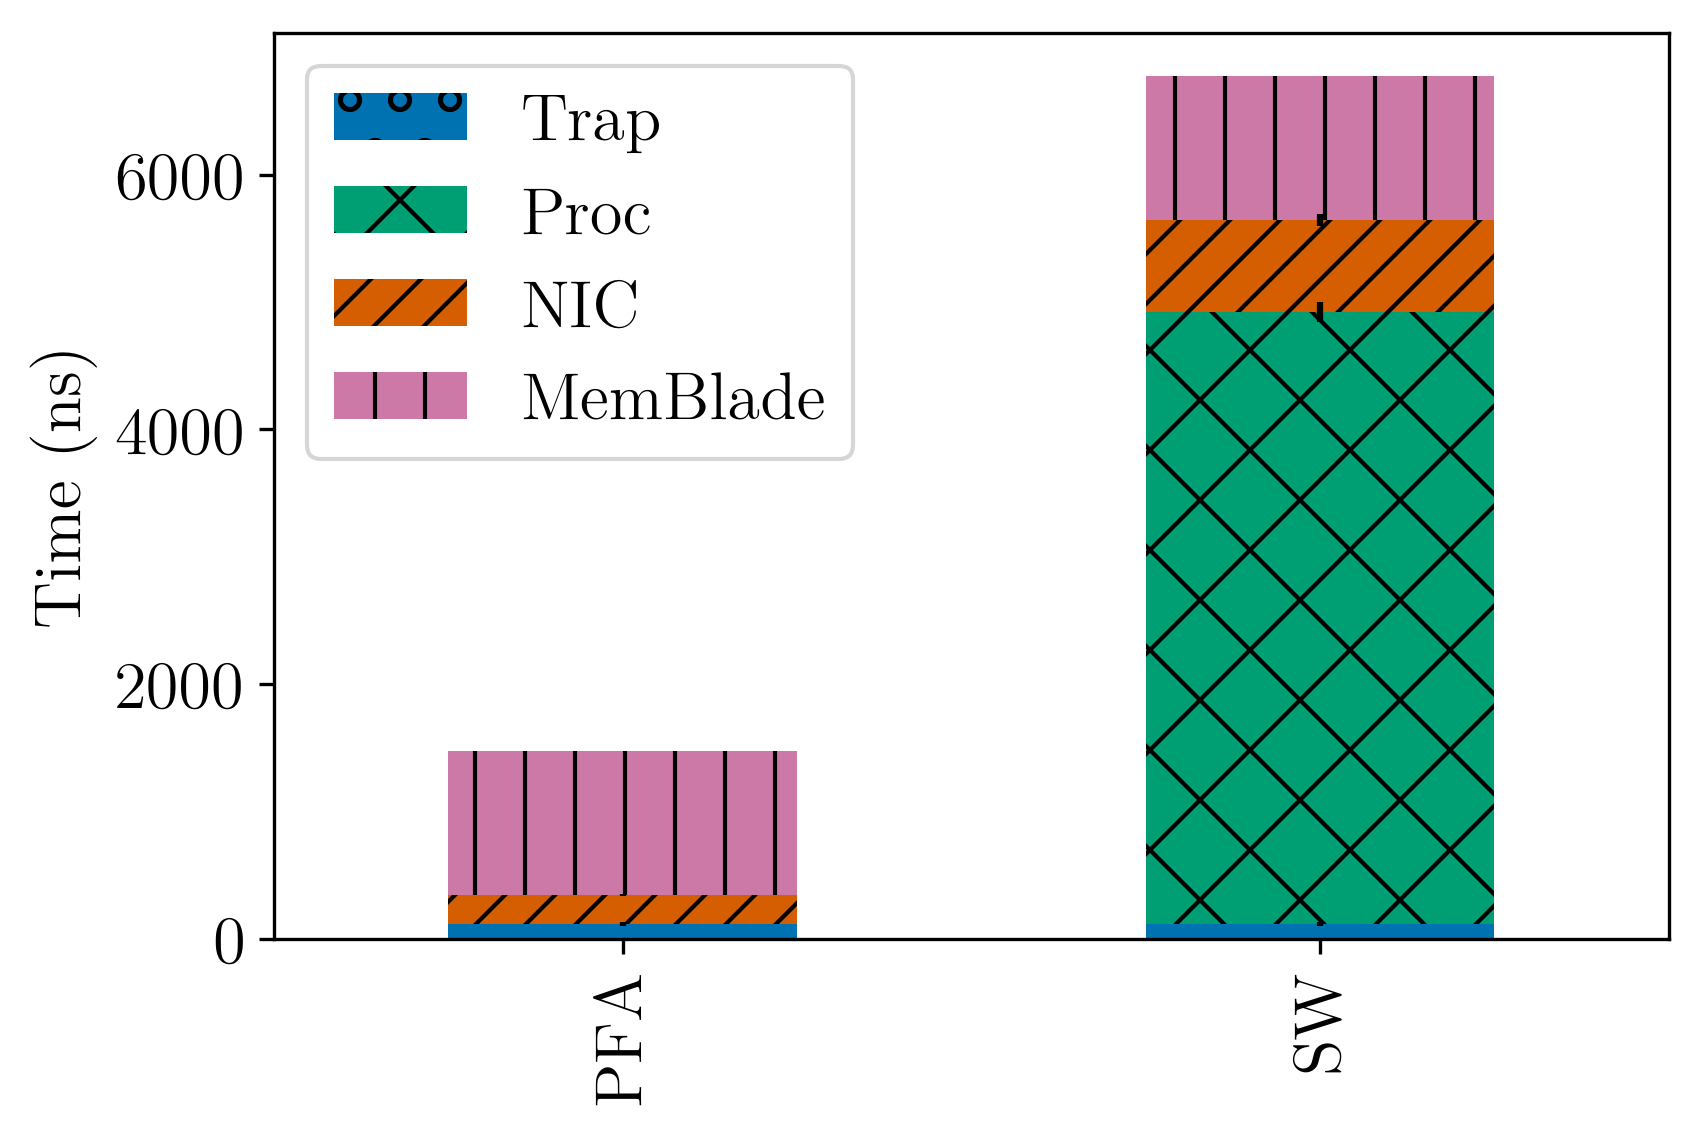
\includegraphics[width=0.8\columnwidth]{figs/fetch_breakdown_fastmem.png}
    \caption{Breakdown of time in fetching a single remote page from a
      hypothetical fast memory blade with \SI{1}{\micro\second} page read
      latency. As network and memory technology improves, the relative benefit
      of the PFA increases (from 2.2x faster with the baseline memory blade to
      4.6x faster with the optimistic memory blade).}
    \label{fig:fetch_breakdown}
  \end{figure}

  \paragraph{Total Page Faults}
  One key function of the PFA is to reduce the number of page faults due to
  paging. Recall from Section \ref{sec:pagingOverview} that there are many
  causes for faults (e.g., to perform copy-on-write), in Figure
  \ref{fig:pfa_swapfault} I plot the number of paging-related faults each
  benchmark experiences as a fraction of total faults. The first thing to note
  is that the number paging-related faults decreases by approximately 64 when
  the PFA is used. This is because the PFA interrupts the OS to perform
  bookkeeping only when its queues are full (every 64 fetches in this
  experiment). However, these only account for 45\% of faults, even in the
  worst-case (our simplest benchmark, Qsort) with 25\% local memory. The more
  complex Gen benchmark has even fewer paging-related faults (as a fraction of
  total). While there are certainly some savings due to fewer kernel crossings,
  they are not frequent nor long enough to explain all the performance benefits
  we see end-to-end.

  \begin{figure}[h] \centering
    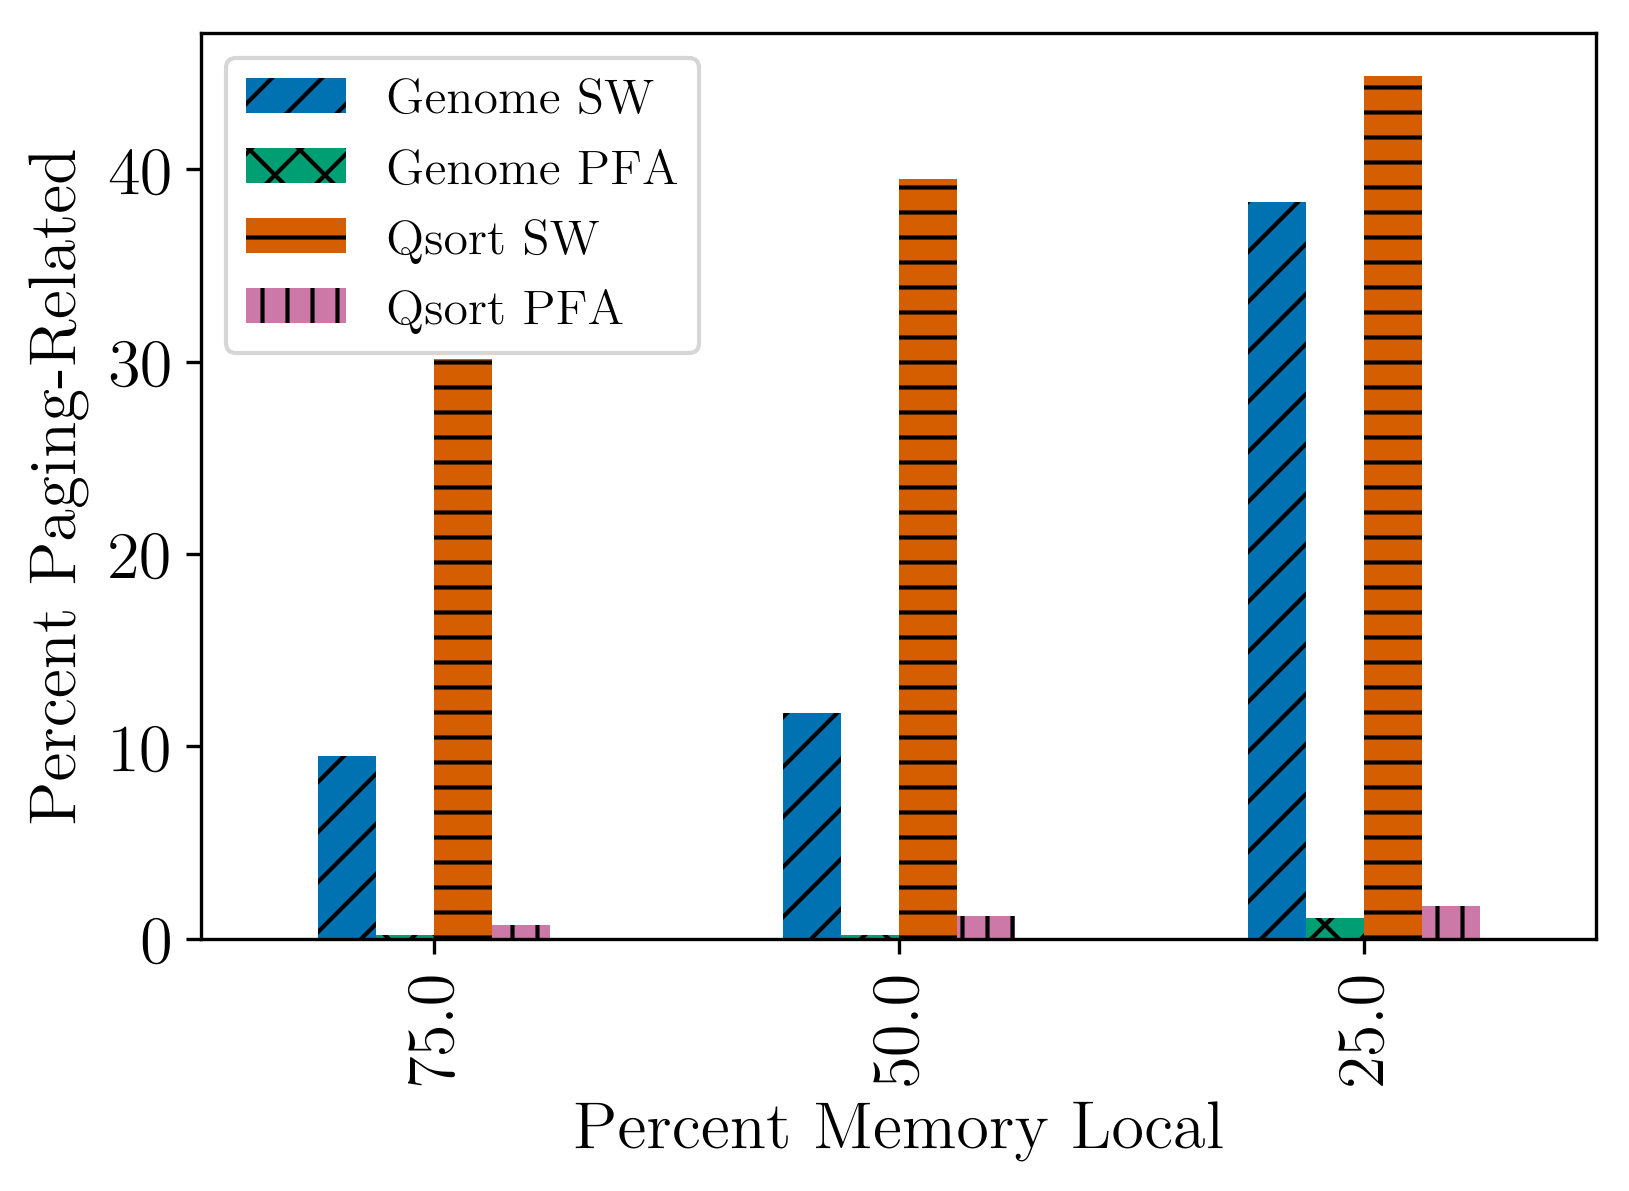
\includegraphics[width=0.9\columnwidth]{figs/swapfault.png}
    \caption{Number of paging-related faults as a fraction of total faults
    experienced.}
    \label{fig:pfa_swapfault}
  \end{figure}

  \paragraph{Bookkeeping Time}
  While we do reduce the number of paging-related faults, the kernel still
  needs to perform bookkeeping on the same number of pages. This batching
  means that more work is performed per page fault with the PFA. Figure
  \ref{fig:pfa_bk_prop} shows total time spent bookkeeping, regardless of the
  number of page faults. What we see is that while the number of evicted pages
  is the same in both configurations, using the PFA leads to a 2.5x reduction
  in bookkeeping time on average. The same code path is executed for each
  new page, but the PFA batches these events, leading to improved cache locality
  for the OS, and fewer cache-polluting page-faults for the application. The
  result is that, even in the worst case, the PFA spends less than half its
  time handling paging-related faults, while the baseline spends about 80\%.

  \begin{figure}[h] \centering
    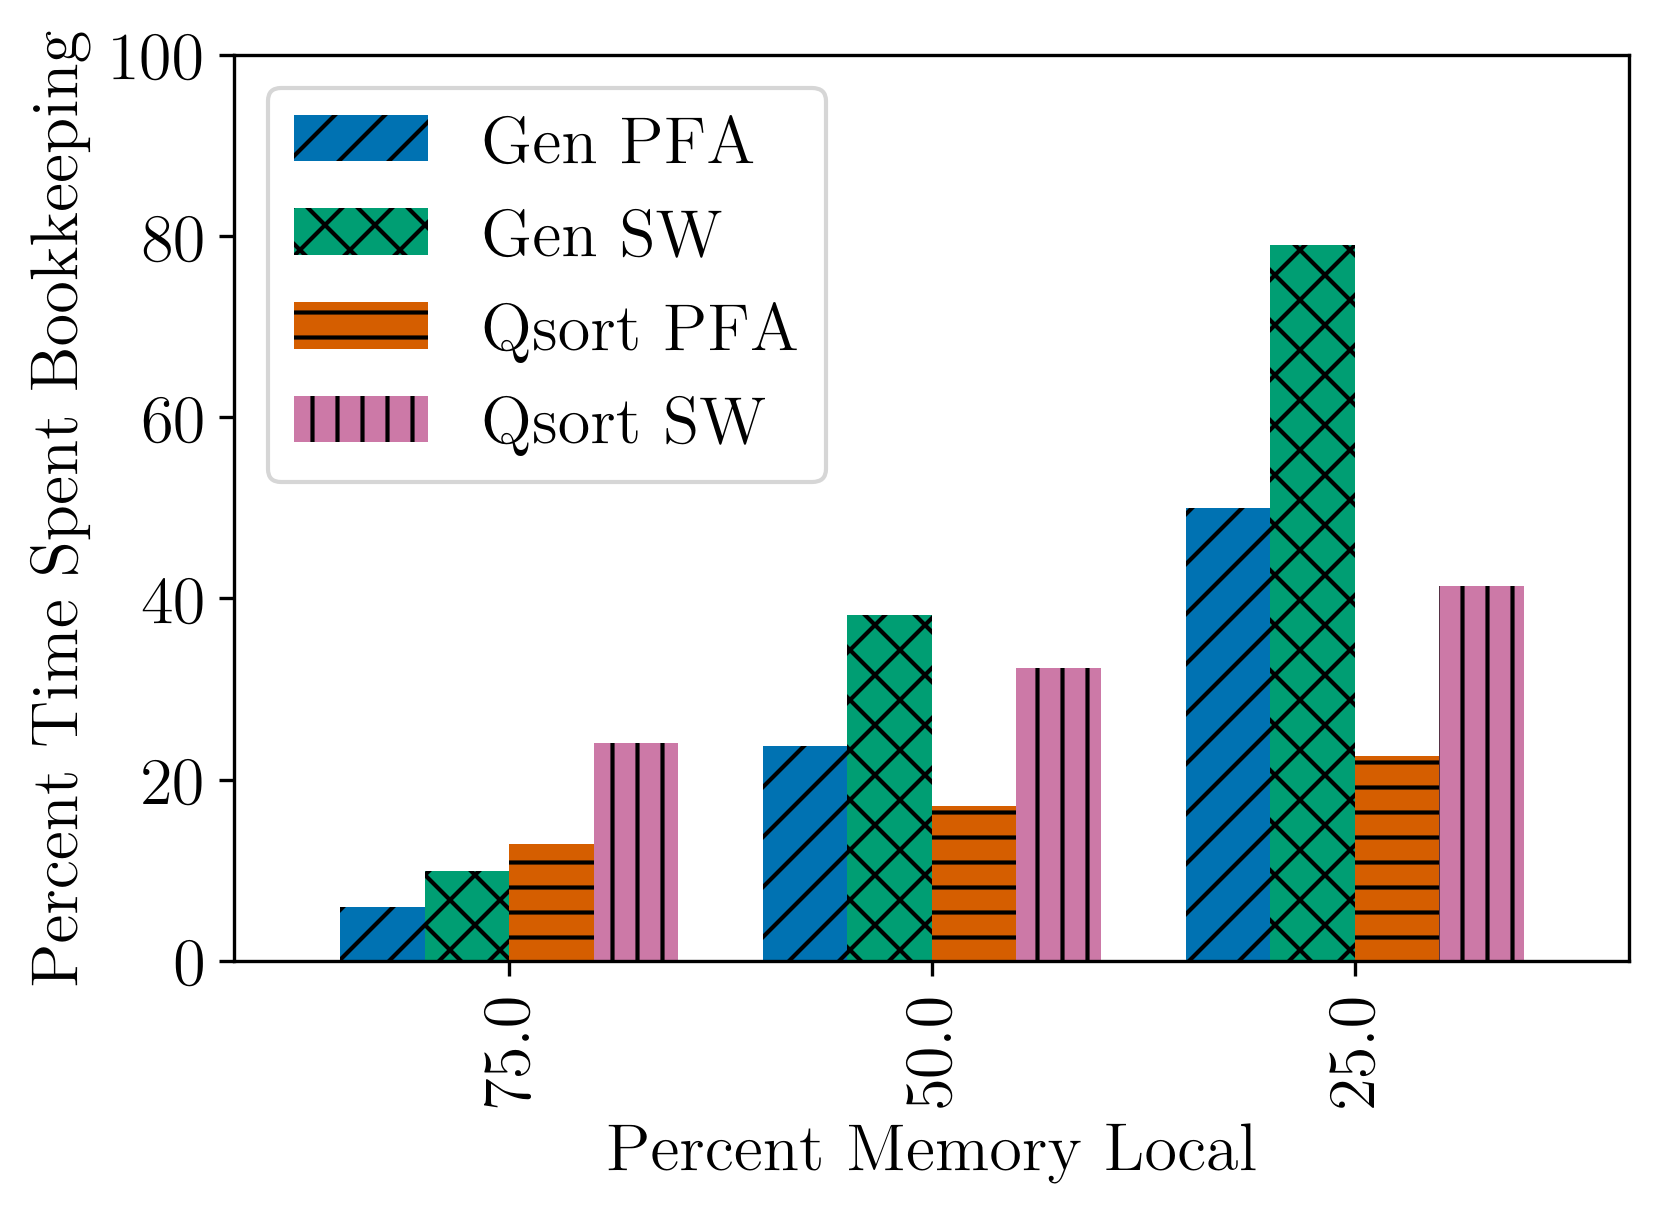
\includegraphics[width=0.8\columnwidth]{figs/bk_prop_all.png}
    \caption{Proportion of Time Spent Bookkeeping}
    \label{fig:pfa_bk_prop}
  \end{figure}

  \paragraph{Scaling}
  Figure \ref{fig:pfa_total_speedup} shows the improvement in end-to-end
  runtime due to the PFA on our applications. While the improvement is
  significant (up to 40\%), the savings are constant (there is no asymptotic
  improvement). This is because the PFA does not change any of the caching
  algorithms, and therefor experiences the same number of faults. This means
  that applications (such as Gen) that are not particularly cache-friendly can
  see significant slowdowns in a disaggregated environment, even with the PFA.
  Ultimately, the PFA pushes the boundaries of what is possible with cache-like
  interfaces, but it cannot change their fundamental limitations. Applications
  like Gen will need deeper changes to be viable on a disaggregated system.

  \begin{figure}[h] \centering
    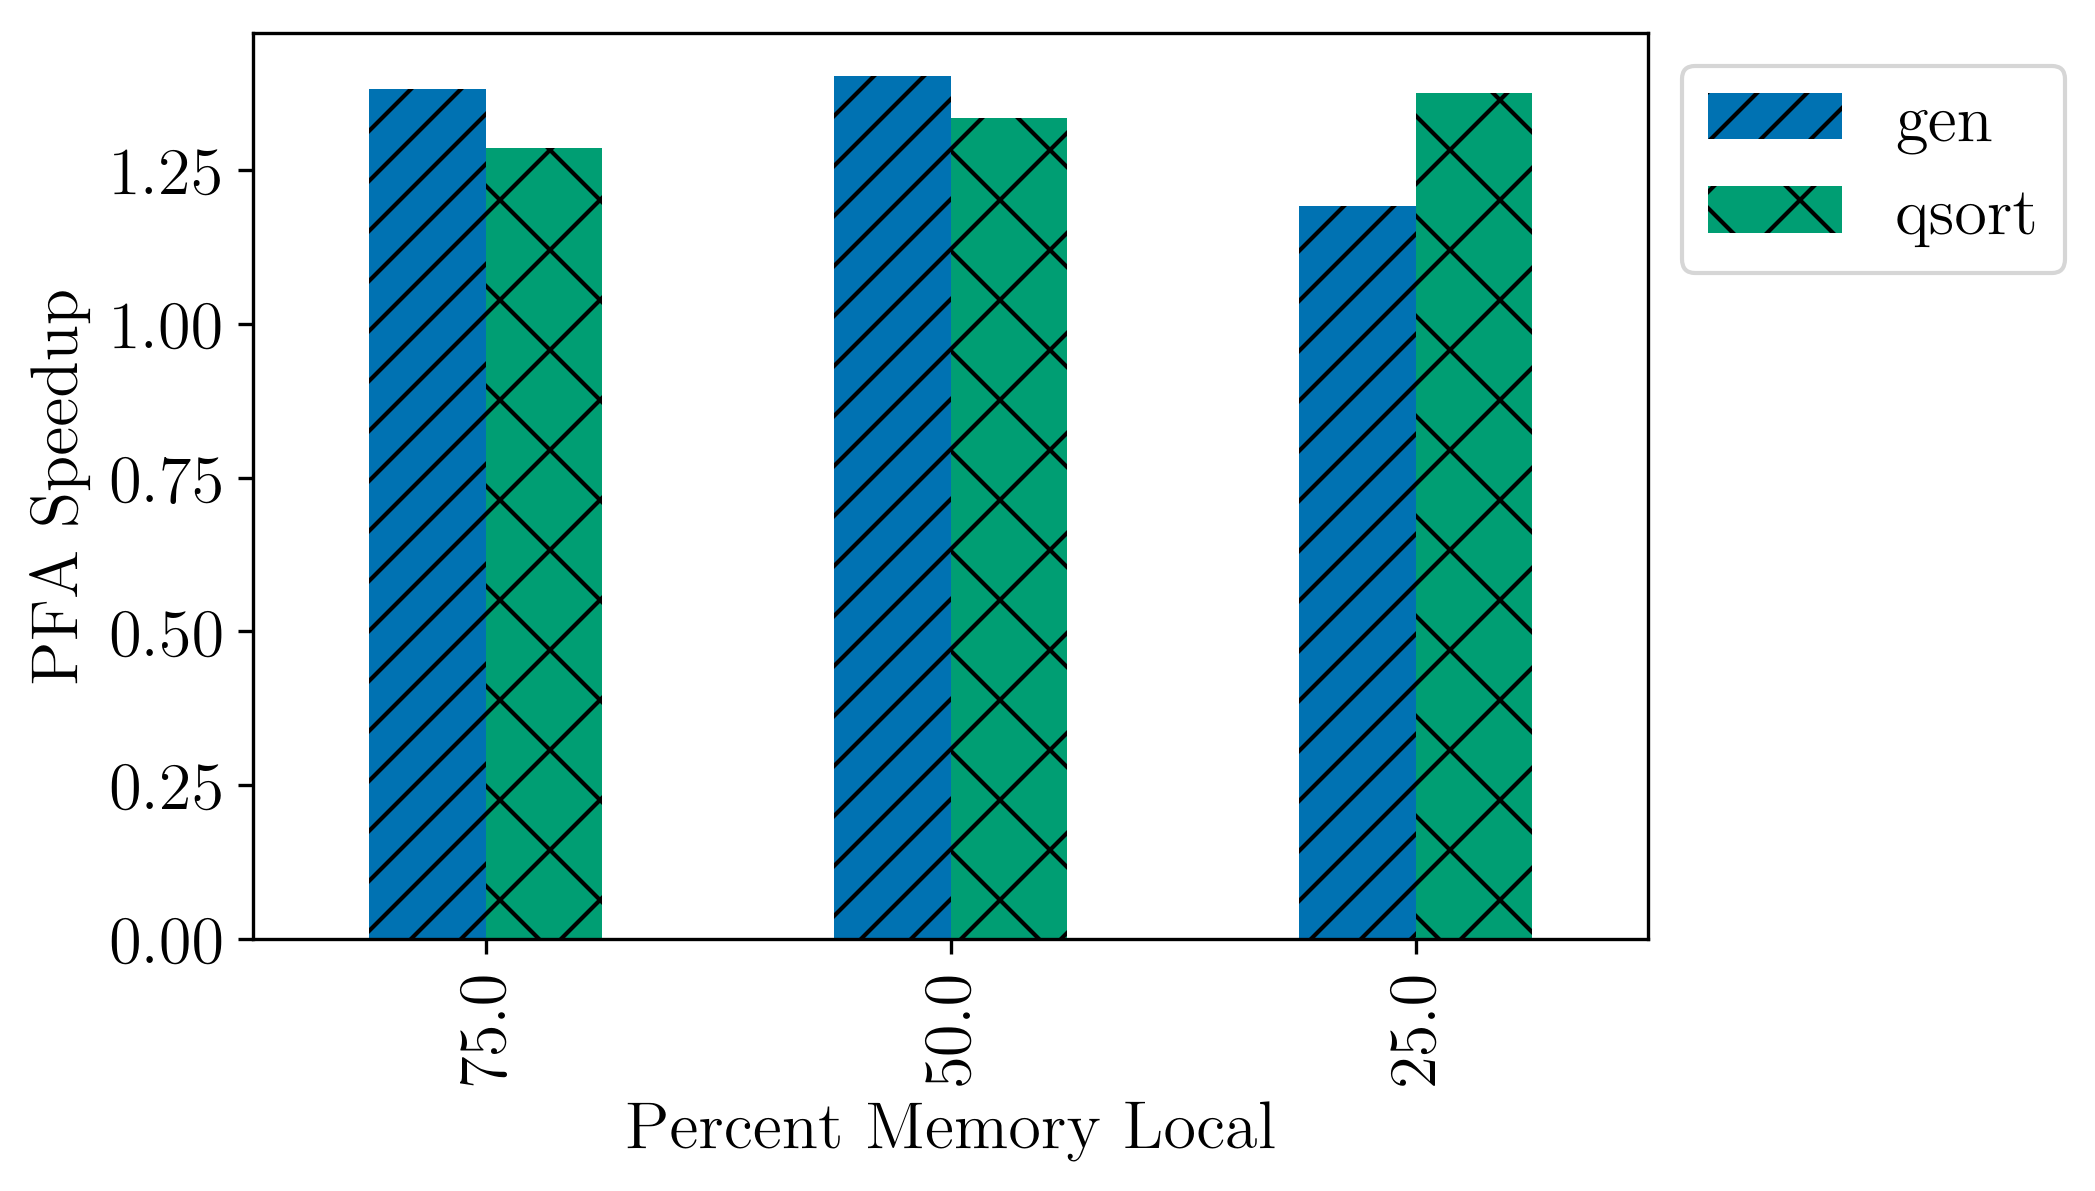
\includegraphics[width=0.8\columnwidth]{figs/total_speedup.png}
    \caption{Total runtime improvement due to PFA}
    \label{fig:pfa_total_speedup}
  \end{figure}



\section{Future Work} \label{sec:future}
    So far, we have only experimented with a single client and memory blade.
However, this does not capture all of the effects that contribute to
performance. In particular, it would be valuable to understand congestion at
both the memory blade, and in the network. Another effect that may surface as
we experiment with more distributed applications is tail latency. The
introduction of a remote page fault could increase tail latency significantly
and would require mitigation.

Another topic not addressed by the current PFA and memory blade designs is that
of management and security. How should memory blade capacity be allocated to
applications? How can such allocations be authenticated? Simple payload
encryption may not be sufficient to protect applications from attackers with
network-level access.

Finally, while caching can be very effective for some workloads, it is not
appropriate everywhere. Even within one workload, caching may be appropriate
for some data structures, but not for others. To allow users maximum
flexibility to choose between performance and convenience, we plan to implement
a hybrid cache/scratchpad interface to remote memory (similar to \cite{vls}).
In this system, application memory would default to demand paging, but certain
portions could be pinned in specially allocated regions of local memory. The
application would then be responsible for directly writing to and from remote
memory.


\section{Conclusion} \label{sec:conclusion}
    Disaggregated memory systems promise to simplify deployment, allocation, and
scheduling on next-generation \glspl{wsc}, but bring significant performance
and complexity challenges. This complexity cannot be mitigated with shallow
application changes because assumptions about system performance run deep.
While caching attempts to avoid these challenges, we find that virtual memory
paging is no different; the OS mechanisms implementing paging were designed in
a world with millisecond-level access latencies and are not suitable for the
microsecond access times offered by remote memory. The PFA allows us to make
the deep changes needed to accommodate this new environment. By improving
end-to-end application performance by up to 40\%, the PFA enables a greater
range of applications to run on limited local memory. However, caching is a
general purpose approach, and applications with large working sets and poor
locality will always suffer from increased main memory access times. To take
full advantage of disaggregated memory, we will need a mix of interfaces, both
implicit, and explicit.



% \listoftodos

\nocite{*}
\newpage
\bibliographystyle{plain}
\bibliography{pfa}

\end{document}
